
\documentclass[UTF8,openany,zihao=-4,oneside]{ctexbook}

% Page and typography
\usepackage[a4paper,top=23mm,bottom=24mm,left=24mm,right=24mm,headheight=15pt,headsep=8mm,footskip=12mm]{geometry}
\linespread{1.08}
\raggedbottom
\sloppy
\emergencystretch=3em

% Core packages
\usepackage{amsmath,amssymb,mathtools}
\usepackage{graphicx}
\graphicspath{{comsol_static_assets/}{comsol_transient_assets/}{comsol_preheater_assets/}}
\usepackage{booktabs,longtable,array,tabularx,multirow,makecell}
\usepackage{enumitem}
\usepackage[table]{xcolor}
\usepackage{tikz}
\usetikzlibrary{positioning,arrows.meta,calc,fit,shapes.geometric}
\usepackage{caption}
\usepackage{float}
\usepackage{fancyhdr}
\usepackage{titlesec}
\usepackage{titletoc}
\usepackage{tocloft}
\usepackage[most]{tcolorbox}
\usepackage{listings}
\usepackage{etoolbox}
\usepackage{hyperref}
\usepackage{bookmark}

% Brand colors
\definecolor{FGBlue}{HTML}{1F4E79}
\definecolor{FGDeep}{HTML}{102A43}
\definecolor{FGCyan}{HTML}{2E8BC0}
\definecolor{FGOrange}{HTML}{D98A15}
\definecolor{FGGray}{HTML}{F3F6F9}
\definecolor{FGLine}{HTML}{D7E2EA}
\definecolor{FGText}{HTML}{243B53}

\hypersetup{
  colorlinks=true,
  linkcolor=FGBlue,
  urlcolor=FGCyan,
  citecolor=FGOrange,
  pdfauthor={FlameGuard},
  pdftitle={稳燃宝 COMSOL 仿真实验设计手册},
  pdfsubject={COMSOL 仿真实验、静态代理、瞬态辨识与预热炉稳态验证},
  pdfkeywords={FlameGuard, 稳燃宝, COMSOL, 焚烧炉, 预热炉, 仿真实验设计}
}

% Paragraph and list tuning
\setlength{\parindent}{2em}
\setlength{\parskip}{0.18em}
\setlist{itemsep=0.15em,topsep=0.35em,leftmargin=2.2em}
\renewcommand{\arraystretch}{1.22}
\setlength{\tabcolsep}{5pt}
\setlength{\LTleft}{0pt}
\setlength{\LTright}{0pt}
\AtBeginEnvironment{longtable}{\small\renewcommand{\arraystretch}{1.2}}

% Pandoc compatibility and manual utilities
\providecommand{\tightlist}{\setlength{\itemsep}{0pt}\setlength{\parskip}{0pt}}
\providecommand{\passthrough}[1]{#1}
\newcommand{\manualdivider}{\par\vspace{0.6em}\noindent\textcolor{FGLine}{\rule{\linewidth}{0.7pt}}\vspace{0.6em}\par}
\newcommand{\pathcode}[1]{\texttt{\detokenize{#1}}}
\newcommand{\notebox}[2]{\begin{tcolorbox}[enhanced,colback=FGBlue!4,colframe=FGBlue!45,boxrule=0.5pt,arc=1.5mm,left=4mm,right=4mm,top=3mm,bottom=3mm]\sffamily\textbf{\color{FGDeep}#1}\par\vspace{0.25em}\color{FGText}#2\end{tcolorbox}}
\newcommand{\warnbox}[2]{\begin{tcolorbox}[enhanced,colback=FGOrange!6,colframe=FGOrange!55,boxrule=0.5pt,arc=1.5mm,left=4mm,right=4mm,top=3mm,bottom=3mm]\sffamily\textbf{\color{FGDeep}#1}\par\vspace{0.25em}\color{FGText}#2\end{tcolorbox}}

% Captions
\captionsetup{font=small,labelfont={bf,color=FGBlue},labelsep=quad}

% Chapter / section styles
\titleformat{\chapter}[display]
  {\Huge\bfseries\sffamily\color{FGDeep}}
  {\begin{tikzpicture}[baseline=(n.base)]\node[fill=FGBlue,text=white,rounded corners=1.5mm,inner xsep=8pt,inner ysep=5pt,font=\Large\bfseries\sffamily] (n) {第\thechapter 章};\end{tikzpicture}}
  {0.85em}
  {\Huge}
  [\vspace{0.35em}{\color{FGOrange}\titlerule[1.2pt]}]
\titlespacing*{\chapter}{0pt}{-4mm}{11mm}

\titleformat{\section}
  {\Large\bfseries\sffamily\color{FGBlue}}
  {\thesection}{0.75em}{}
  [\vspace{0.15em}{\color{FGLine}\titlerule[0.6pt]}]
\titlespacing*{\section}{0pt}{2.1ex plus .4ex}{1.1ex}

\titleformat{\subsection}
  {\large\bfseries\sffamily\color{FGDeep}}
  {\thesubsection}{0.75em}{}
\titlespacing*{\subsection}{0pt}{1.8ex plus .3ex}{0.8ex}

\titleformat{\subsubsection}
  {\normalsize\bfseries\sffamily\color{FGDeep}}
  {\thesubsubsection}{0.65em}{}
\titlespacing*{\subsubsection}{0pt}{1.3ex plus .2ex}{0.55ex}

% TOC styling
\renewcommand{\cftchapfont}{\sffamily\bfseries\color{FGDeep}}
\renewcommand{\cftsecfont}{\sffamily\color{FGText}}
\renewcommand{\cftchappagefont}{\sffamily\bfseries\color{FGBlue}}
\renewcommand{\cftsecpagefont}{\sffamily\color{FGText}}
\setlength{\cftbeforechapskip}{0.45em}

% Header / footer
\pagestyle{fancy}
\fancyhf{}
\fancyhead[L]{\sffamily\small\color{FGDeep}“稳燃宝”COMSOL 仿真实验设计手册}
\fancyhead[R]{\sffamily\small\color{FGBlue}\leftmark}
\fancyfoot[L]{\sffamily\scriptsize\color{FGText}静态扫描 · 瞬态辨识 · 预热稳定性验证}
\fancyfoot[R]{\sffamily\small\bfseries\color{FGBlue}\thepage}
\renewcommand{\headrulewidth}{0.5pt}
\renewcommand{\footrulewidth}{0pt}
\renewcommand{\headrule}{\hbox to\headwidth{\color{FGLine}\leaders\hrule height \headrulewidth\hfill}}
\fancypagestyle{plain}{%
  \fancyhf{}%
  \fancyfoot[R]{\sffamily\small\bfseries\color{FGBlue}\thepage}%
  \renewcommand{\headrulewidth}{0pt}%
}

% Code listings
\lstdefinestyle{fgcode}{
  basicstyle=\ttfamily\small,
  backgroundcolor=\color{FGGray},
  frame=single,
  rulecolor=\color{FGLine},
  framerule=0.5pt,
  breaklines=true,
  columns=fullflexible,
  keepspaces=true,
  showstringspaces=false,
  tabsize=2,
  xleftmargin=1em,
  xrightmargin=1em,
  framexleftmargin=0.6em,
  framexrightmargin=0.6em,
  aboveskip=0.8em,
  belowskip=0.8em
}
\lstset{style=fgcode}

% Inline badges, aligned with the other manuals
\newcommand{\fgbadge}[1]{\tcbox[colback=FGBlue!6,colframe=FGBlue!35,boxrule=0.4pt,arc=1mm,left=2pt,right=2pt,top=1pt,bottom=1pt,on line]{\sffamily\footnotesize #1}}

\begin{document}

\begin{titlepage}
\begin{tikzpicture}[remember picture,overlay]
  \fill[FGDeep] (current page.north west) rectangle ([yshift=-88mm]current page.north east);
  \fill[FGBlue] ([yshift=-88mm]current page.north west) rectangle ([yshift=-92mm]current page.north east);
  \fill[FGOrange] ([yshift=-92mm]current page.north west) rectangle ([yshift=-94mm]current page.north east);
  \fill[FGGray] ([yshift=-94mm]current page.north west) rectangle (current page.south east);
  \draw[FGBlue!20,line width=1.2pt] ([xshift=18mm,yshift=-122mm]current page.north west) -- ([xshift=-18mm,yshift=-122mm]current page.north east);
\end{tikzpicture}
\vspace*{13mm}
{\sffamily\bfseries\color{white}\fontsize{18}{22}\selectfont FlameGuard / 稳燃宝}\par
\vspace{9mm}
{\sffamily\bfseries\color{white}\fontsize{31}{38}\selectfont COMSOL 仿真实验设计手册}\par
\vspace{4mm}
{\sffamily\color{white}\fontsize{15}{20}\selectfont 焚烧炉静态代理 · 焚烧炉动态辨识 · 预热炉温度稳定性验证}\par
\vspace{36mm}
\begin{tcolorbox}[enhanced,width=\textwidth,colback=white,colframe=FGLine,boxrule=0.7pt,arc=2mm,drop shadow={black!12!white},left=8mm,right=8mm,top=6mm,bottom=6mm]
{\sffamily\bfseries\Large\color{FGDeep}v0.2.0 Beta}\par\vspace{0.6em}
\end{tcolorbox}
\vfill
{\sffamily\small\color{FGText}炉火纯青队 · 大学生节能减排社会实践与科技竞赛 · 2025}\par
\end{titlepage}

\frontmatter
\pagestyle{plain}
\tableofcontents
\cleardoublepage
\pagestyle{fancy}
\mainmatter

\chapter{概述}

本手册用于介绍“稳燃宝”（FlameGuard）项目中 COMSOL 仿真的实验设计。包括边界条件、输入输出变量、数据处理方式和与 Python 控制框架的接口关系。

\notebox{实验对象}{目前已经完成的 COMSOL 仿真分为三类：第一，焚烧炉静态参数扫描，用于建立干基垃圾质量流量、入口含水率与焚烧炉输出及烟气资源之间的稳态关系；第二，焚烧炉瞬态仿真，用于辨识静态关系之外的响应延迟和惯性；第三，预热炉静态仿真，用于验证给定预热工况下温度场稳定性和热边界是否满足控制系统要求。}

COMSOL 结果进入控制框架时，应遵循项目已有接口：控制器向被控对象发送 \pathcode{PlantStepInput(command, feedstock, dt)}；COMSOL backend 将 \pathcode{ActuatorCommand} 转换为 \(T_g\)、\(v_g\) 或等效边界条件，将 \pathcode{FeedstockObservation} 转换为入口含水率、干基质量流量和热物性；求解完成后返回 \pathcode{PlantSnapshot}。最小返回内容为 \(T_{avg}\)、\(T_{stack}\) 和 \(v_{stack}\)，若可输出预热炉出口或沿程状态，应进一步返回 \pathcode{PreheaterOutput} 或 \pathcode{PreheaterState}。

\manualdivider


\chapter{焚烧炉静态仿真实验}

为了建模焚烧炉燃烧特性，即燃烧区域温度、温度稳定性、烟囱烟气物料性质与进入焚烧炉的垃圾质量及其含水率的关系，由 COMSOL Multiphysics 6.4 建立三维稳态非等温湍流模型，采用“固体和流体传热 + 湍流，代数 $y^+$ + 非等温流动”耦合，用于获得进入焚烧炉的干基垃圾质量流量和湿基含水率对燃烧区域温度、燃烧面温度分布、烟囱排气温度与排气速度的影响。

\section{模型对象与几何边界}

COMSOL 模型以主燃区、过渡段、上升烟道和烟囱为主体，并保留外壁固体区域，用于同时计算炉内气相流动、固体壁面导热和外壁散热。几何采用 SI 单位，报告统计为 18 个域、92 个边界、152 条边和 80 个顶点。主要结构参数如表 \ref{tab:furnace-geom-param} 所示。

\begin{table}[htbp]
\centering\footnotesize
\begin{tabularx}{\textwidth}{p{25mm}p{23mm}p{23mm}X}
\toprule
结构部位 & 参数 & 数值 & 说明 \\
\midrule
主燃区 & $D_1,H_1$ & $1.4\ \mathrm{m},\ 1.8\ \mathrm{m}$ & 炉膛主体直径和高度。\\
燃烧区域 & $H_{burn}$ & $0.63\ \mathrm{m}$ & 由 $H_1\times0.35$ 给出，是体积热源施加区域。\\
进气区域 & $H_{airin}$ & $0.09\ \mathrm{m}$ & 由 $H_1\times0.05$ 给出，入口温度和法向速度边界位于该区域底部边界。\\
过渡段 & $D_2,H_2$ & $1.0\ \mathrm{m},\ 1.6\ \mathrm{m}$ & 连接主燃区与上升烟道。\\
上升烟道 & $D_3,H_3$ & $0.8\ \mathrm{m},\ 0.3\ \mathrm{m}$ & 烟气由主燃区过渡至烟囱前的收缩段。\\
烟囱 & $D_4,H_4$ & $0.6\ \mathrm{m},\ 7.5\ \mathrm{m}$ & 输出烟囱温度和烟囱轴向速度的主要评价位置。\\
壁厚设置 & 外半径增量 & 分段设置 & 主燃区、过渡段、上升烟道和烟囱外半径分别增加 $0.10$、$0.08$、$0.05$、$0.03\ \mathrm{m}$。\\
\bottomrule
\end{tabularx}
\caption{焚烧炉静态 COMSOL 模型的主要几何参数}
\label{tab:furnace-geom-param}
\end{table}

\begin{figure}[htbp]
\centering
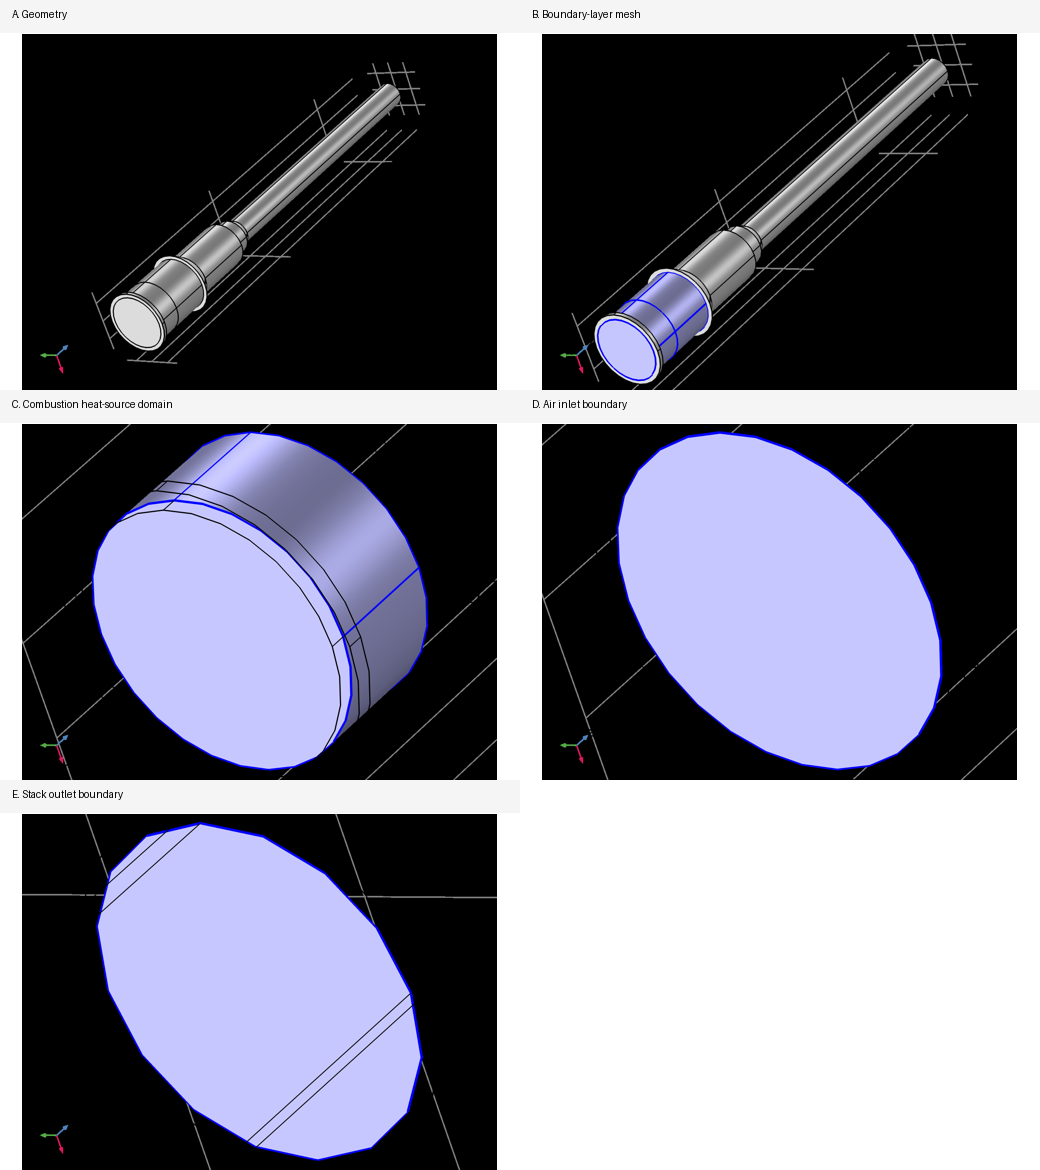
\includegraphics[width=0.78\textwidth]{geometry_physics_montage.png}
\caption{焚烧炉静态仿真的几何、网格与主要物理边界。A 为整体几何，B 为边界层网格设置，C 为主燃区体积热源区域，D 为进气边界，E 为烟囱出口压力边界。}
\label{fig:furnace-static-geometry}
\end{figure}

\section{物理场、材料与边界条件}

模型使用三类材料：气相域为空气，金属结构域采用 304 不锈钢，耐火/保温结构域采用 36\% 孔隙率莫来石材料。流动部分使用弱可压缩湍流模型，湍流模型为 RANS-EVM 框架下的代数 $y^+$ 模型，壁面处理采用自动壁处理；传热部分同时包含流体传热、固体传热、体积热源、入口定温、外壁对流散热和非等温流动耦合。

\begin{table}[htbp]
\centering\small
\begin{tabularx}{\textwidth}{p{31mm}p{40mm}X}
\toprule
设置项 & COMSOL 报告设置 & 手册中的工程含义 \\
\midrule
气相入口 & 边界 15；法向流入速度 $u_{in}$；入口温度 $T_{in}=293.15\ \mathrm{K}$ & 将燃烧空气和等效生成气体折算为入口质量流率，再由入口面积换算为法向速度。\\
烟囱出口 & 边界 56；压力 $0\ \mathrm{Pa}$；抑制回流开启 & 用于得到烟囱出口平均温度和轴向速度，作为后续预热炉可用烟气资源边界。\\
主燃区热源 & 域 6；体积热源 $Q$ & 将干基垃圾低位热值、水分等效吸热和燃烧区域体积折算为体积放热率。\\
外壁散热 1 & 对流热通量；$h=10\ \mathrm{W/(m^2\cdot K)}$；$T_{amb}=293.15\ \mathrm{K}$ & 表征一般外壁自然/弱强制对流散热。\\
外壁散热 2 & 对流热通量；$h=15\ \mathrm{W/(m^2\cdot K)}$；$T_{amb}=293.15\ \mathrm{K}$ & 对部分更强换热边界单独提高传热系数。\\
非等温耦合 & Kays-Crawford 湍流普朗特数模型；标准热壁函数；包含黏性耗散 & 使速度场、温度场和气体物性在稳态计算中相互耦合。\\
\bottomrule
\end{tabularx}
\caption{焚烧炉静态仿真的主要物理场与边界条件}
\label{tab:furnace-static-physics}
\end{table}

网格采用物理场控制网格并叠加局部尺寸控制。全局最大单元尺寸为 1.18 m，最小单元尺寸为 0.0284 m；流体域局部最大单元尺寸为 0.165 m，局部最小单元尺寸为 0.0284 m；关键边界进一步收紧到最小单元尺寸 0.01062 m；流体壁面设置 6 层边界层，厚度调节因子为 2。该设置的重点不是追求几何全域等尺寸加密，而是保证炉膛、收缩段和烟囱内壁附近的速度梯度、温度梯度和壁面函数计算稳定。

\section{参数化扫描与热量折算}

本实验的两个自变量为干基质量扫描倍率 $r_d$ 和进入焚烧炉湿基含水率 $w_b$。COMSOL 报告中采用所有组合扫描：
\[
 r_d\in\{0.5,1.0,1.5,2.0,2.5,3.0,3.5\},\qquad
 w_b\in\{0,10,20,30,40,50\}\ .
\]
因此总计形成 42 个稳态工况。$w_b$ 在报告中以百分数保存，进入公式时换算为 $\omega_b=w_b/100$。干基质量流量由基准预热炉入口湿垃圾质量流率和基准预热炉入口含水率反推：
\[
\dot m_{pre,ref}=\frac{20000}{86400}=0.23148\ \mathrm{kg/s},\qquad
\omega_{pre,ref}=0.77535,
\]
\[
\dot m_{d,ref}=(1-\omega_{pre,ref})\dot m_{pre,ref}=0.052002\ \mathrm{kg/s},\qquad
\dot m_d=r_d\dot m_{d,ref}.
\]
水分质量流量、湿垃圾质量流量和净放热功率为：
\[
\dot m_w=\dot m_d\frac{\omega_b}{1-\omega_b},\qquad
\dot m_b=\dot m_d+\dot m_w,
\]
\[
Q_{comb}=\dot m_d LHV_d,\qquad
Q_{water}=\dot m_wH_{water},\qquad
Q_{net}=\eta_Q(Q_{comb}-Q_{water}).
\]
其中 $H_{water}=4.0\times10^6\ \mathrm{J/kg}$，$LHV_d=1.2049\times10^7\ \mathrm{J/kg}$，$\eta_Q=1$。体积热源通过核心燃烧区域体积 $V_{core}=0.96981\ \mathrm{m^3}$ 转换为：
\[
Q=\frac{Q_{net}}{V_{core}}.
\]
空气供给使用空气系数 $\lambda=1.6$。理论空气质量流率和实际助燃空气质量流率分别为：
\[
\dot m_{air,st}=\alpha_{air,E}Q_{comb},\qquad
\dot m_{air}=\lambda\dot m_{air,st},
\]
其中 $\alpha_{air,E}=0.35\ \mathrm{kg/MJ}$。等效生成气体质量流率为 $\dot m_{prod}=1.8\dot m_d+\dot m_w$，等效入口气体质量流率为 $\dot m_{gas,eff}=\dot m_{air}+\dot m_{prod}$，入口速度为：
\[
 u_{in}=\frac{\dot m_{gas,eff}}{\rho_{in}A_{in}},\qquad
 A_{in}=1.5394\ \mathrm{m^2}.
\]

这个折算方式的意义在于：$r_d$ 主要改变干基可燃物放热量、理论空气量、生成气体量和烟囱速度；$w_b$ 主要通过水分等效吸热项降低净放热量，同时也改变湿垃圾质量和生成气体质量。由此，静态仿真可以直接给出“含水率扰动”和“干基负荷扰动”对温度场和烟气资源的不同影响。

\section{派生量与结果表格}

COMSOL 报告输出 6 个用于控制器代理建模的派生量，分别对应表格 23 至表格 28。原始温度均为 K；进入控制器文档和代理拟合时，温度水平量换算为 $^\circ\mathrm{C}$，而温度标准差属于温差量，数值在 K 与 $^\circ\mathrm{C}$ 下相同。

\begin{table}[htbp]
\centering\small
\begin{tabularx}{\textwidth}{p{31mm}p{30mm}p{24mm}X}
\toprule
COMSOL 派生量 & 手册变量 & 单位 & 用途 \\
\midrule
燃烧区域平均温度 & $T_{avg}$ & $^\circ\mathrm{C}$ & 判断炉膛主体温度是否满足稳定燃烧和控制约束。\\
表面最大值 1 & $T_{surface,max}$ & $^\circ\mathrm{C}$ & 评价燃烧面局部高温和耐火材料安全裕度。\\
表面最小值 1 & $T_{surface,min}$ & $^\circ\mathrm{C}$ & 识别局部低温、冷斑和不完全燃烧风险。\\
面标准差 1 & $\sigma_T$ & $^\circ\mathrm{C}$（温差） & 表征燃烧面温度均匀性。\\
表面平均 6 & $T_{stack}$ & $^\circ\mathrm{C}$ & 烟囱排气温度，用于预热炉可用热资源估计。\\
表面平均 7 & $v_{stack}$ & $\mathrm{m/s}$ & 烟囱轴向速度，用于烟气流量和资源边界估计。\\
\bottomrule
\end{tabularx}
\caption{COMSOL 派生量与控制器静态代理变量的对应关系}
\label{tab:furnace-derived-values}
\end{table}

代表性工况结果见表 \ref{tab:furnace-static-representative}。其中 $r_d=1,w_b=20\%$ 为报告中的基准进入焚烧炉工况；高湿工况显示出明显降温趋势，说明预热炉脱水效果对主炉稳定燃烧具有直接影响。

\begin{table}[htbp]
\centering\small
\begin{tabular}{rrrrrrr}
\toprule
$r_d$ & $w_b$/\% & $T_{avg}$/\(^\circ\mathrm{C}\) & $T_{stack}$/\(^\circ\mathrm{C}\) & $v_{stack}$/m/s & $T_{surf,min}$/\(^\circ\mathrm{C}\) & $T_{surf,max}$/\(^\circ\mathrm{C}\) \\
\midrule
0.5 & 20 & 912.65 & 864.15 & 2.6335 & 590.61 & 1143.65 \\
1.0 & 20 & 927.15 & 932.75 & 5.5747 & 721.67 & 1147.95 \\
2.0 & 20 & 937.05 & 995.35 & 11.7010 & 863.55 & 1153.25 \\
3.5 & 20 & 941.85 & 1040.15 & 21.1700 & 984.65 & 1155.35 \\
1.0 & 40 & 769.25 & 777.55 & 5.0856 & 597.39 & 952.35 \\
1.0 & 50 & 649.72 & 659.06 & 4.6737 & 504.55 & 804.55 \\
\bottomrule
\end{tabular}
\caption{焚烧炉静态参数扫描的代表性工况结果}
\label{tab:furnace-static-representative}
\end{table}

\begin{figure}[htbp]
\centering
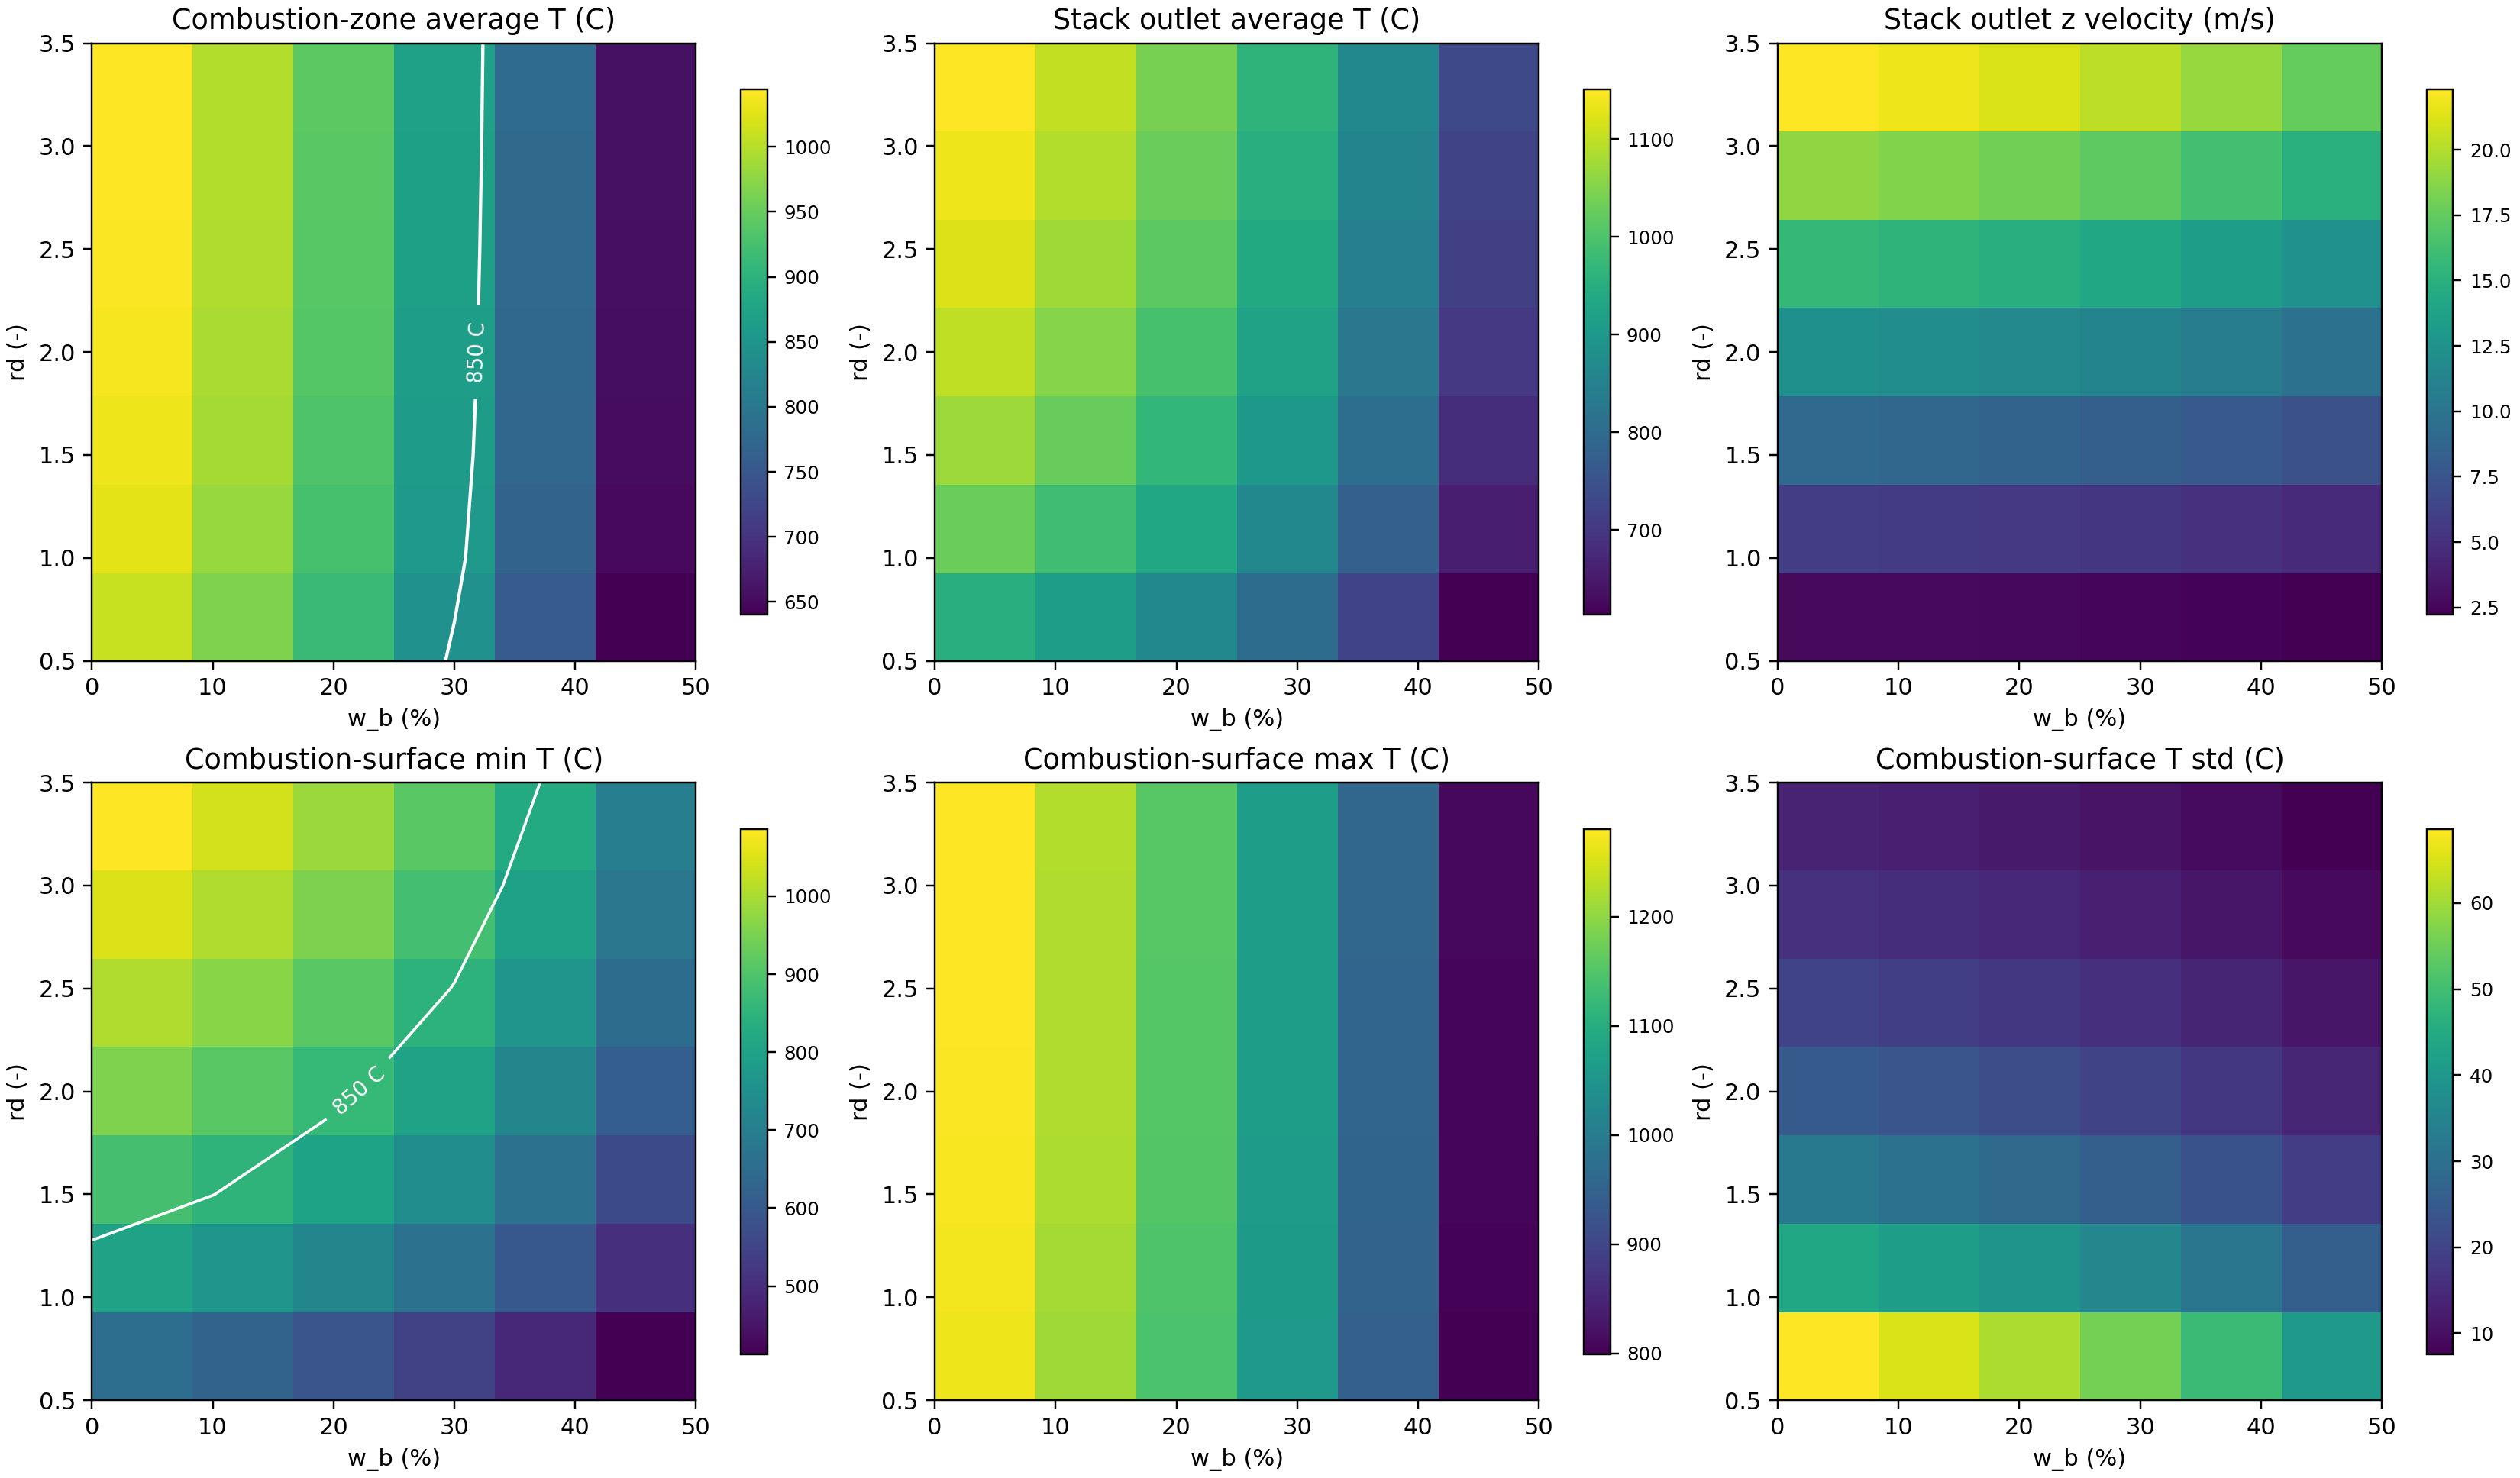
\includegraphics[width=0.98\textwidth]{furnace_static_heatmaps.png}
\caption{焚烧炉静态批量扫描结果热图。横轴为湿基含水率 $w_b$，纵轴为干基质量倍率 $r_d$。白色等值线标出 $850^\circ\mathrm{C}$ 参考线，用于观察平均炉温和燃烧面最低温度的安全边界。}
\label{fig:furnace-static-heatmaps}
\end{figure}

\section{结果规律与工程解释}

从批量扫描结果可以提取出三条直接服务于控制器设计的结论。

第一，湿基含水率是炉膛平均温度的主导扰动。以 $r_d=1$ 为例，$w_b$ 从 0\% 增加到 50\% 时，$T_{avg}$ 从 $1027.05^\circ\mathrm{C}$ 降至 $649.72^\circ\mathrm{C}$，下降约 $377.33^\circ\mathrm{C}$；同一过程中 $T_{stack}$ 从 $1030.25^\circ\mathrm{C}$ 降至 $659.06^\circ\mathrm{C}$。这说明若预热炉未能充分脱水，主焚烧炉难以仅通过增加干基负荷维持高温区间。

第二，干基质量倍率对烟囱速度和烟气资源的影响强于对炉膛平均温度的影响。以 $w_b=20\%$ 为例，$r_d$ 从 0.5 增加到 3.5 时，$T_{avg}$ 仅从 $912.65^\circ\mathrm{C}$ 升至 $941.85^\circ\mathrm{C}$，增加约 $29.20^\circ\mathrm{C}$；但 $T_{stack}$ 从 $864.15^\circ\mathrm{C}$ 升至 $1040.15^\circ\mathrm{C}$，$v_{stack}$ 从 2.6335 m/s 升至 21.1700 m/s。因此，$r_d$ 更适合作为烟气资源、排烟速度和处理负荷的主要驱动量，而不是作为抵消高含水率冲击的唯一调节量。

第三，燃烧面最低温度比燃烧区域平均温度更加严格。虽然部分工况下 $T_{avg}$ 可维持在 $850^\circ\mathrm{C}$ 以上，但 $T_{surface,min}$ 仍可能显著低于该阈值。例如基准工况 $r_d=1,w_b=20\%$ 下，$T_{avg}=927.15^\circ\mathrm{C}$，但 $T_{surface,min}=721.67^\circ\mathrm{C}$。因此，控制器不宜只以区域平均温度作为唯一安全指标，应至少将 $T_{surface,min}$ 或等效冷斑风险指标作为高保真校核项。

\begin{figure}[htbp]
\centering
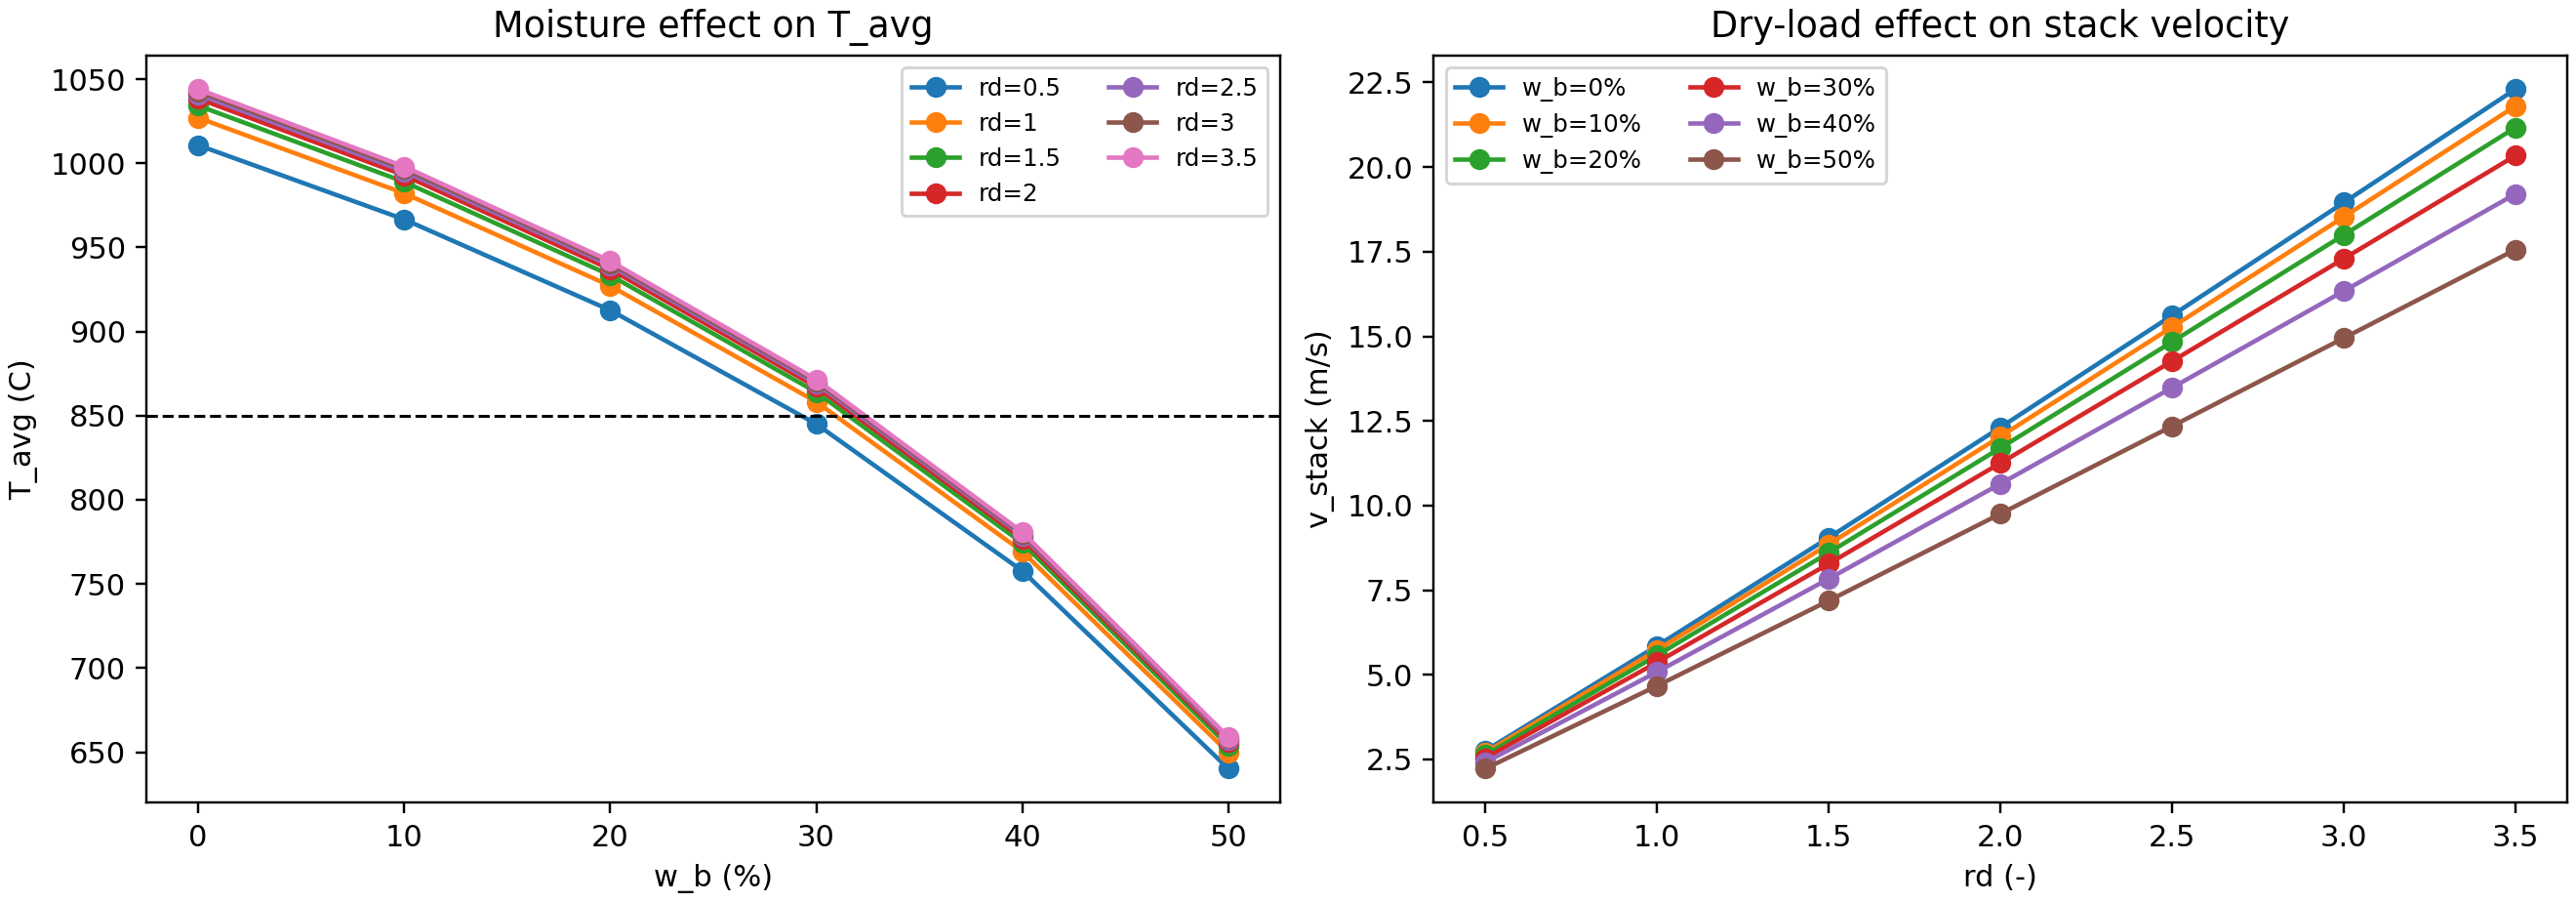
\includegraphics[width=0.88\textwidth]{furnace_static_sensitivity_lines.png}
\caption{典型灵敏度曲线。左图显示含水率升高导致炉膛平均温度快速下降；右图显示干基质量倍率升高显著提高烟囱轴向速度。}
\label{fig:furnace-static-sensitivity}
\end{figure}

COMSOL 报告中的三维场图进一步说明，主燃区和过渡段存在明显温度梯度，烟囱段则承担了温度场和速度场向出口边界发展的作用。该结果支持当前手册中将焚烧炉静态模型拆分为“炉膛温度指标”和“烟气资源指标”的做法。

\begin{figure}[htbp]
\centering
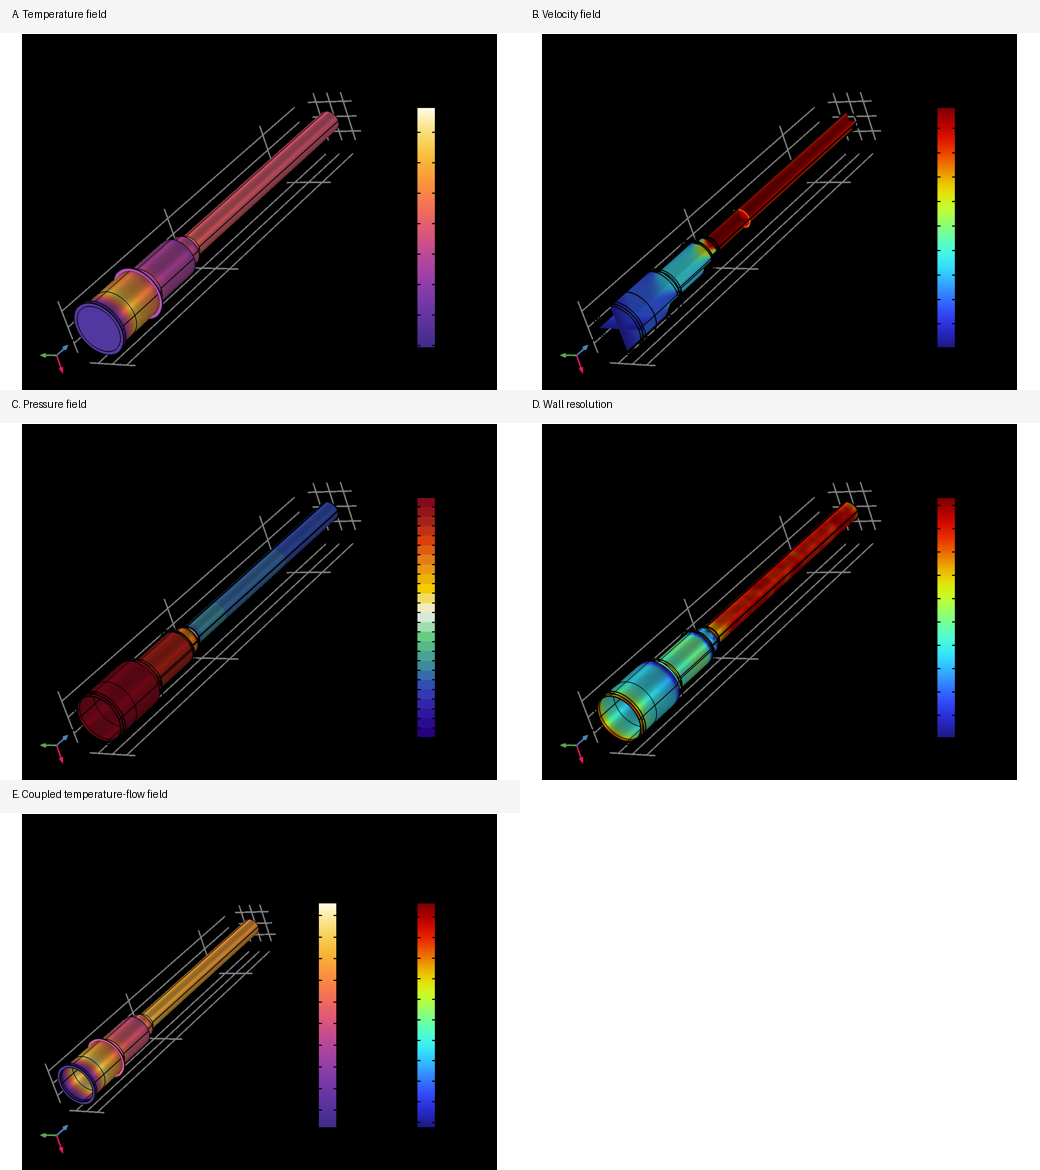
\includegraphics[width=0.96\textwidth]{comsol_fields_montage.png}
\caption{COMSOL 报告中的典型三维结果图。温度、速度、压力、壁面分辨率和非等温流动耦合结果共同用于判断模型是否存在局部异常、出口回流或壁面解析不足。}
\label{fig:furnace-static-fields}
\end{figure}


\section{与静态代理模型的衔接}

静态 COMSOL 扫描结果整理为规则表格，并拟合为可在毫秒级调用的静态代理。当前项目脚本 \pathcode{scripts/fit_furnace_static_surrogate.py} 的输入为 6 个 COMSOL 表格导出的 CSV 文件，每个文件包含 \pathcode{rd,w_b,value} 三列；其中 \pathcode{w_b} 为湿基含水率百分数，温度型输出在脚本中由 K 自动换算为 $^\circ\mathrm{C}$，烟囱速度和温度标准差则保持原数值量纲。

本次补充运行得到的拟合文件为 \pathcode{scripts/furnace_static_surrogate_fit.json}。拟合采用以中心点平移后的二维三阶总次数多项式，中心点和模型阶数为：
\[
 x=r_d-3.0,\qquad z=\omega_b-0.3218,\qquad \deg=3.
\]
对任一输出 $Y_j$，代理形式为：
\[
Y_j=\sum_{(a,b)\in\mathcal P}c_{j,a,b}x^az^b,
\]
其中
\[
\mathcal P=\{(0,0),(0,1),(0,2),(0,3),(1,0),(1,1),(1,2),(2,0),(2,1),(3,0)\}.
\]
因此每个输出量包含 10 个系数。6 个输出量分别为炉膛平均温度、烟囱排气温度、烟囱排气速度、燃烧面最低温度、燃烧面最高温度和燃烧面温度标准差；每个输出均由 42 个 COMSOL 工况点拟合得到。

\begin{lstlisting}[language=bash,caption={焚烧炉静态代理拟合脚本运行命令与主要输出},label={lst:furnace-surrogate-fit-run}]
python scripts/fit_furnace_static_surrogate.py
wrote scripts/furnace_static_surrogate_fit.json
degree=3 terms=10
T_avg_C            train_rmse=0.7627 train_max=1.94  loo_rmse=1.009 loo_max=2.294
T_stack_C          train_rmse=2.223  train_max=5.806 loo_rmse=3.065 loo_max=7.008
v_stack_mps        train_rmse=0.02121 train_max=0.05809 loo_rmse=0.03239 loo_max=0.08264
T_surface_min_C    train_rmse=3.679  train_max=9.051 loo_rmse=5.26  loo_max=11.99
T_surface_max_C    train_rmse=0.7083 train_max=1.189 loo_rmse=0.9416 loo_max=1.814
T_surface_std_C    train_rmse=0.7838 train_max=1.983 loo_rmse=1.086 loo_max=2.763
\end{lstlisting}

\begin{table}[htbp]
\centering\small
\begin{tabular}{lrrrrr}
\toprule
输出量 & 训练 RMSE & 训练最大误差 & LOO RMSE & LOO 最大误差 & 样本数 \\
\midrule
$T_{avg}$ / $^\circ\mathrm{C}$ & 0.763 & 1.940 & 1.009 & 2.294 & 42 \\
$T_{stack}$ / $^\circ\mathrm{C}$ & 2.223 & 5.806 & 3.065 & 7.008 & 42 \\
$v_{stack}$ / m/s & 0.021 & 0.058 & 0.032 & 0.083 & 42 \\
$T_{surface,min}$ / $^\circ\mathrm{C}$ & 3.679 & 9.051 & 5.260 & 11.993 & 42 \\
$T_{surface,max}$ / $^\circ\mathrm{C}$ & 0.708 & 1.189 & 0.942 & 1.814 & 42 \\
$\sigma_T$ / $^\circ\mathrm{C}$ & 0.784 & 1.983 & 1.086 & 2.763 & 42 \\
\bottomrule
\end{tabular}
\caption{焚烧炉静态代理拟合误差与留一交叉验证结果}
\label{tab:furnace-surrogate-error}
\end{table}

\begin{figure}[htbp]
\centering
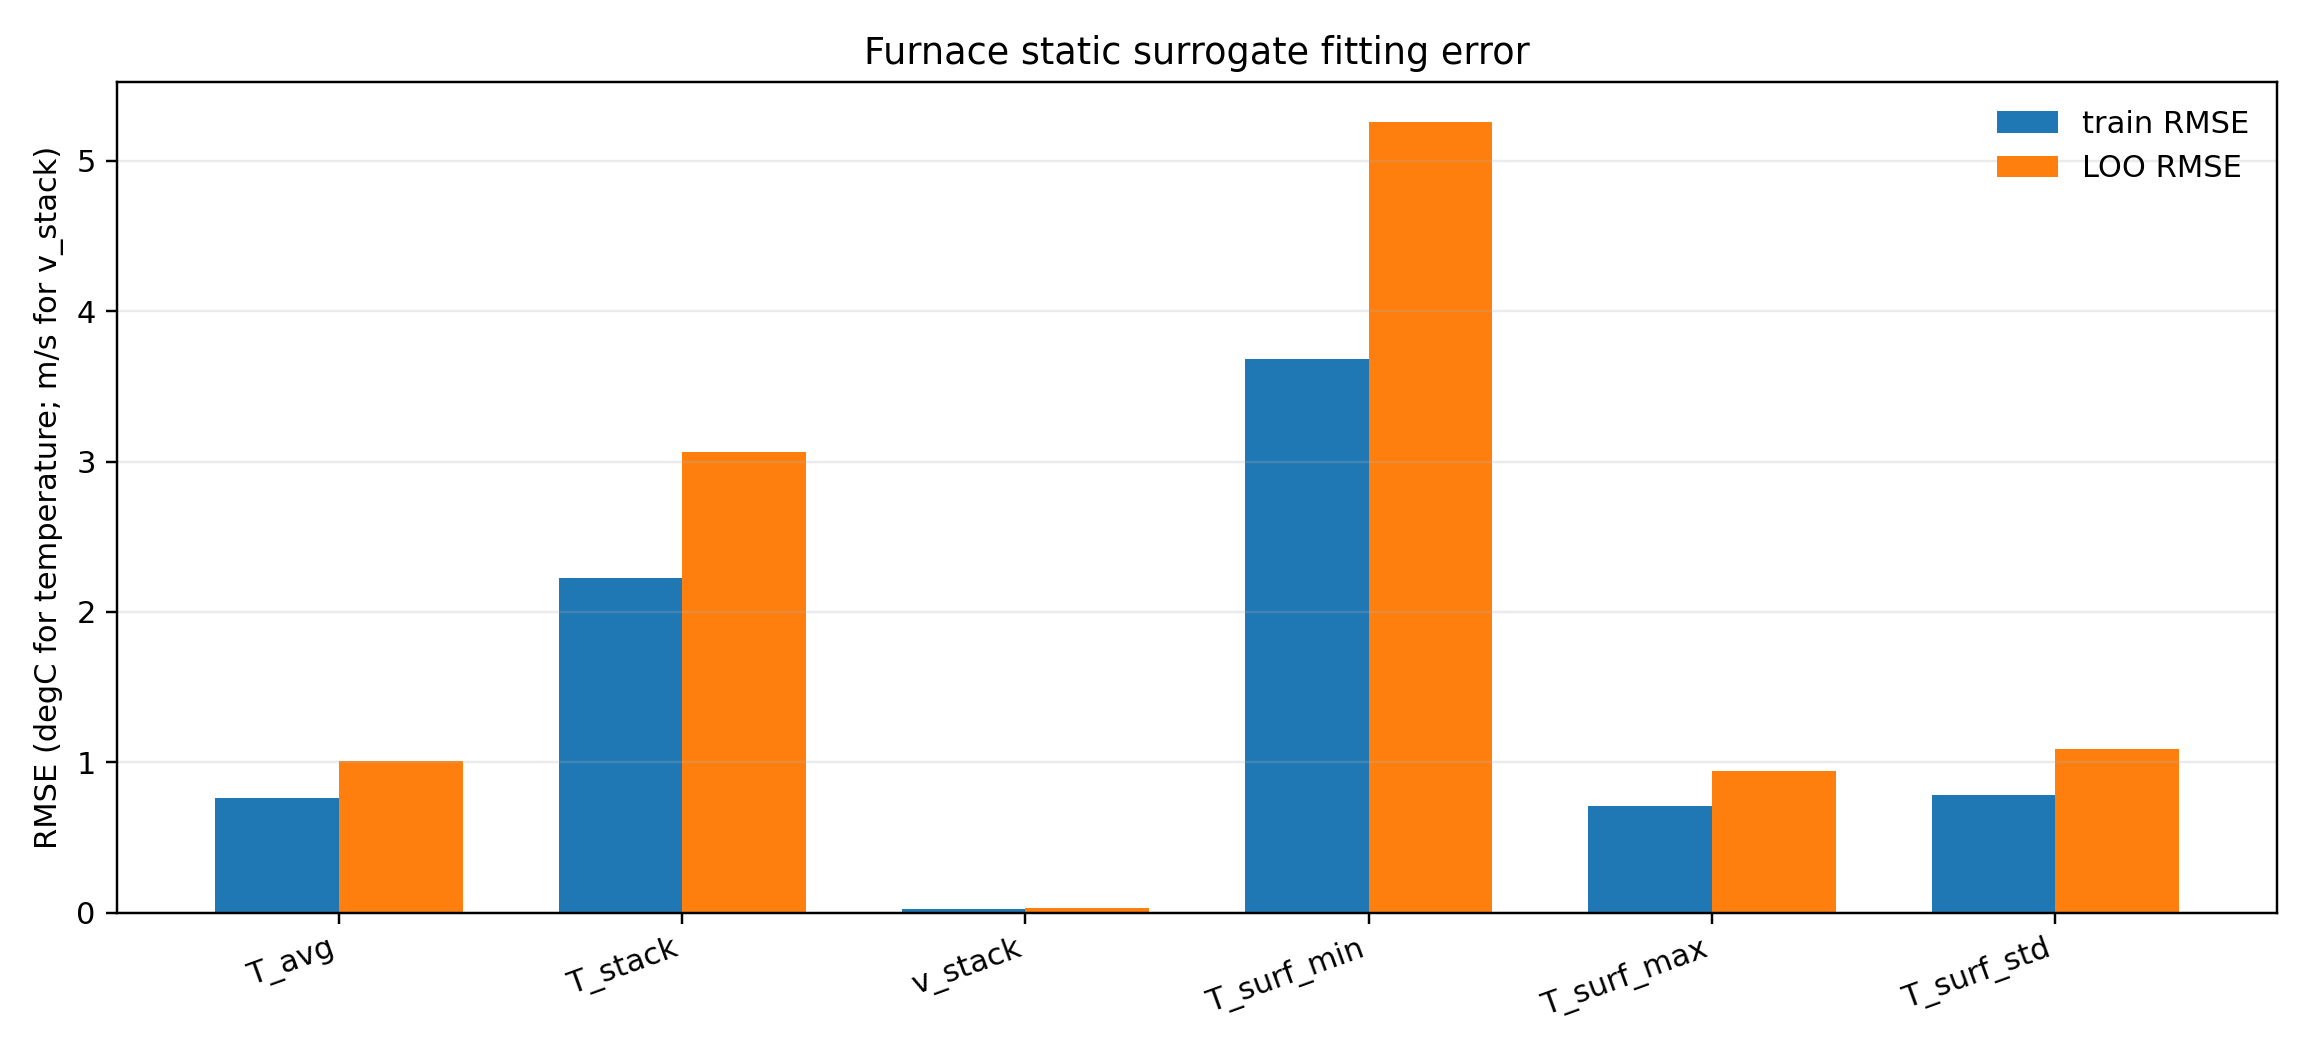
\includegraphics[width=0.95\textwidth]{furnace_surrogate_error_bars.png}
\caption{焚烧炉静态代理拟合误差对比。温度相关通道的误差单位为 $^\circ\mathrm{C}$，烟囱速度通道的误差单位为 m/s，图中仅用于比较各通道训练误差与留一交叉验证误差的相对变化。}
\label{fig:furnace-surrogate-error-bars}
\end{figure}

从拟合质量看，炉膛平均温度、燃烧面最高温度和燃烧面温度标准差的代理误差较小，其中 $T_{avg}$ 的留一 RMSE 约为 $1.01^\circ\mathrm{C}$，$T_{surface,max}$ 的留一 RMSE 约为 $0.94^\circ\mathrm{C}$。烟囱排气温度的留一 RMSE 约为 $3.07^\circ\mathrm{C}$，对后续烟气热资源估算而言仍属于较低误差水平。烟囱排气速度的留一 RMSE 为 $0.032\ \mathrm{m/s}$，最大留一误差为 $0.083\ \mathrm{m/s}$，可满足控制器对烟气资源变化趋势的估计需求。

燃烧面最低温度 $T_{surface,min}$ 是误差最大的通道，留一 RMSE 为 $5.26^\circ\mathrm{C}$，最大留一误差约 $11.99^\circ\mathrm{C}$。这与冷斑位置对局部流动、燃烧区域分布和含水率变化更敏感有关。因此，在控制器中使用该量作为安全约束或冷斑风险指标时，不宜只使用代理预测值本身，而应保留至少 $10$--$15^\circ\mathrm{C}$ 的保守裕度；若后续要把燃烧面最低温度作为硬约束，建议增加高含水率、低干基负荷边界附近的 COMSOL 样本点，或对 $T_{surface,min}$ 单独采用分段/局部加权代理。

\begin{table}[htbp]
\centering\small
\begin{tabular}{lrrr}
\toprule
输出量 & $c_{0,0}$ & $c_{0,1}$：含水率一阶项 & $c_{1,0}$：干基倍率一阶项 \\
\midrule
$T_{avg}$ & 852.443 & -849.481 & 2.467 \\
$T_{stack}$ & 932.440 & -919.254 & 23.535 \\
$v_{stack}$ & 17.104 & -9.067 & 5.991 \\
$T_{surface,min}$ & 864.466 & -834.140 & 66.613 \\
$T_{surface,max}$ & 1047.382 & -1039.730 & 1.386 \\
$\sigma_T$ & 13.539 & -13.989 & -5.138 \\
\bottomrule
\end{tabular}
\caption{中心点附近的主要代理系数摘要}
\label{tab:furnace-surrogate-coeff-main}
\end{table}

表 \ref{tab:furnace-surrogate-coeff-main} 只摘录常数项、含水率一阶项和干基倍率一阶项，用于解释中心点附近的主导趋势，不替代完整 JSON 系数。可以看出，含水率一阶项在温度通道中均为明显负值，说明在中心点附近提高入口湿基含水率会显著降低炉膛和燃烧面温度；干基倍率一阶项对烟囱速度和燃烧面最低温度更敏感，说明垃圾负荷提高不仅改变热释放水平，也会提高排烟速度和局部燃烧面下限温度。由于模型包含高阶项，上述一阶系数只能解释中心点附近的局部趋势，边界工况仍应以完整多项式预测结果为准。

\manualdivider


\chapter{焚烧炉瞬态仿真实验}

静态代理模型给出了焚烧炉在给定入口含水率和干基负荷下的稳态输出，但控制器还需要知道的是入口扰动进入炉膛后的响应速度、滞后和混合过程。因此进行焚烧炉瞬态仿真实验，被认为可能对实验结果具有影响的变量包括：垃圾离开预热炉到进入焚烧炉之间的延迟过程、垃圾在焚烧炉内与已有垃圾的混合效应、炉体及固体热容。

\warnbox{注意}{为了保证求解收敛，对延迟与混合效应的 COMSOL 仿真未采用完整湍流多物理场耦合，因此温度、速度等绝对数值不作为静态代理模型的校准依据；本章只使用其中的动态结构，即含水率阶跃、低位热值变化、体热源变化、延迟环节和核心区混合环节。}

\section{材料组成与仿真用途}

本章使用的两个 COMSOL 报告均基于同一焚烧炉几何骨架：主燃区直径为 \(1.4\,\mathrm{m}\)，主燃区高度为 \(1.8\,\mathrm{m}\)，过渡段直径为 \(1.0\,\mathrm{m}\)，上升烟道直径为 \(0.8\,\mathrm{m}\)，烟囱直径为 \(0.6\,\mathrm{m}\)，烟囱高度为 \(7.5\,\mathrm{m}\)。入口速度设置为 \(0.8\,\mathrm{m/s}\)，入口温度和环境温度均为 \(293.15\,\mathrm{K}\)。进料质量流率取 \(20000\,\mathrm{kg}/86400\,\mathrm{s}=0.23148\,\mathrm{kg/s}\)，核心燃烧区域体积为 \(0.96981\,\mathrm{m^3}\)。

\begin{table}[htbp]
\centering\small
\begin{tabularx}{\textwidth}{p{34mm}p{37mm}X}
\toprule
材料 & 主要设置 & 在本手册中的用途 \\
\midrule
瞬态材料 & 固体与流体传热；为收敛未使用完整湍流多物理场；含水率阶跃；包含全局 ODE 延迟与混合环节 & 证明预热炉出口含水率变化不会瞬时作用到燃烧区，而是经过运输延迟和核心区库存混合后进入等效热源。 \\
热容效应材料 & 固体与流体传热、湍流代数 \(y^+\)、非等温流动耦合；包含炉体/固体材料热容 & 检查炉体热容是否在 100--600 s 量级内成为控制器预测的主导动态。 \\
静态扫描材料 & 完整静态参数扫描与三阶多项式拟合 & 提供最终稳态面 \(F(\omega_b,r_d)\)，仍作为温度和烟气资源绝对数值的主要来源。 \\
\bottomrule
\end{tabularx}
\caption{焚烧炉瞬态材料与静态代理材料的分工}
\end{table}

图 \ref{fig:transient-model-montage} 给出了瞬态模型中的阶跃函数、几何、网格和温度场示意。无湍流瞬态材料的网格包含 18088 个网格顶点、88008 个四面体单元、25586 个三角形单元，最小单元质量为 0.1754，平均单元质量为 0.6295。热容效应模型为了处理湍流和边界层，网格规模增大到 79028 个网格顶点、175491 个四面体单元和 91476 个棱柱单元，总单元数为 266967，平均单元质量为 0.7182。由此也可以看出，热容效应验证是更重的补充算例，而不是后续在线控制器可直接调用的求解形式。

\begin{figure}[htbp]
\centering
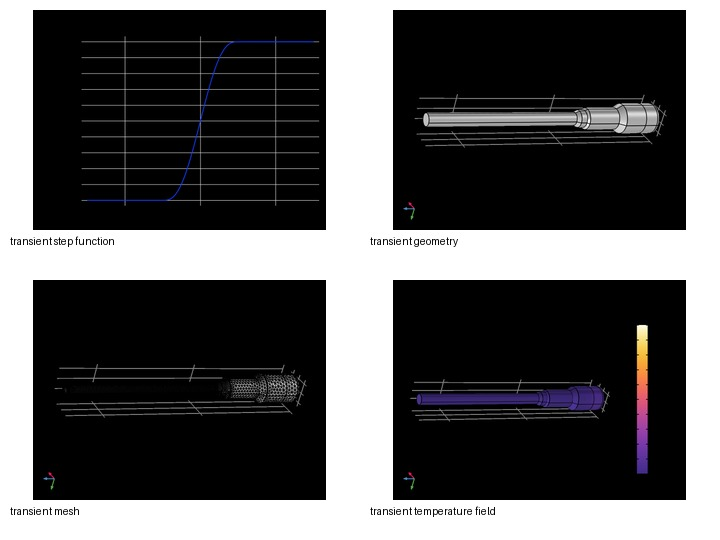
\includegraphics[width=0.94\textwidth]{transient_model_montage.jpg}
\caption{焚烧炉瞬态材料中的阶跃函数、几何、网格和温度场示意}
\label{fig:transient-model-montage}
\end{figure}

\section{动态含水率、低位热值与体热源设置}

瞬态材料将预热炉出口含水率视为扰动输入，初始湿基含水率为 \(w_0=20\%\)，阶跃幅值为 \(\Delta w=20\%\)。无湍流瞬态材料中报告参数给出的阶跃位置为 200 s；热容效应材料中阶跃位置为 100 s。由于两份材料的目标不同，本手册不把阶跃时刻作为固定工程参数，而把其理解为“用于激发焚烧炉动态响应的含水率扰动”。

预热炉输出理想含水率写为：
\[
w_{out}=w_0+\Delta w\,\mathrm{step}(t)
\]
COMSOL 中低位热值与等效体热源采用：
\[
LHV=(3498+118.7(65-w))\times 10^3\ \mathrm{J/kg}
\]
\[
Q=\frac{\dot m\,LHV}{V_{core}}
\]
其中 \(\dot m=0.23148\,\mathrm{kg/s}\)，\(V_{core}=0.96981\,\mathrm{m^3}\)。这意味着含水率阶跃并不是直接施加为温度边界，而是先改变湿基低位热值，再通过核心燃烧区体热源影响炉膛温度场。该处理与静态代理模型中的物理逻辑一致：入口含水率升高会降低等效热释放，进而降低 \(T_{avg}\)、\(T_{stack}\) 和燃烧面温度。

\section{延迟与混合环节}

无湍流瞬态材料中的关键不是温度绝对值，而是全局常微分方程。报告中设置两个状态变量 \(x_1\) 和 \(x_2\)，其中 \(x_1\) 表征预热炉出口含水率到达主燃区前的延迟环节，\(x_2\) 表征核心燃烧区内有效平均含水率。方程可整理为：
\[
\frac{dx_1}{dt}=\frac{w_{out}-x_1}{\tau_{trans}},\qquad \tau_{trans}=5\,\mathrm{s}
\]
\[
\frac{dx_2}{dt}=\frac{x_1-x_2}{\tau_{mix}},\qquad \tau_{mix}=\frac{M_{mix}}{\dot m}=75.412\,\mathrm{s}
\]
其中
\[
M_{mix}=\rho_b\beta_{mix}V_{core}=450\times0.04\times0.96981=17.457\,\mathrm{kg}
\]
因此，进入燃烧区热源计算的不是理想阶跃含水率 \(w_{out}\)，而是经过快速输运延迟和慢速库存混合后的 \(w_{eff}=x_2\)。图 \ref{fig:ode-moisture-response} 按报告参数重构了该动态过程。可以看到，\(x_1\) 在数秒内接近阶跃输入，而 \(x_2\) 受核心区有效库存质量控制，需要约一个 \(\tau_{mix}\) 的时间达到 63.2\% 响应，并在数百秒内逐步接近新稳态。

\begin{figure}[htbp]
\centering
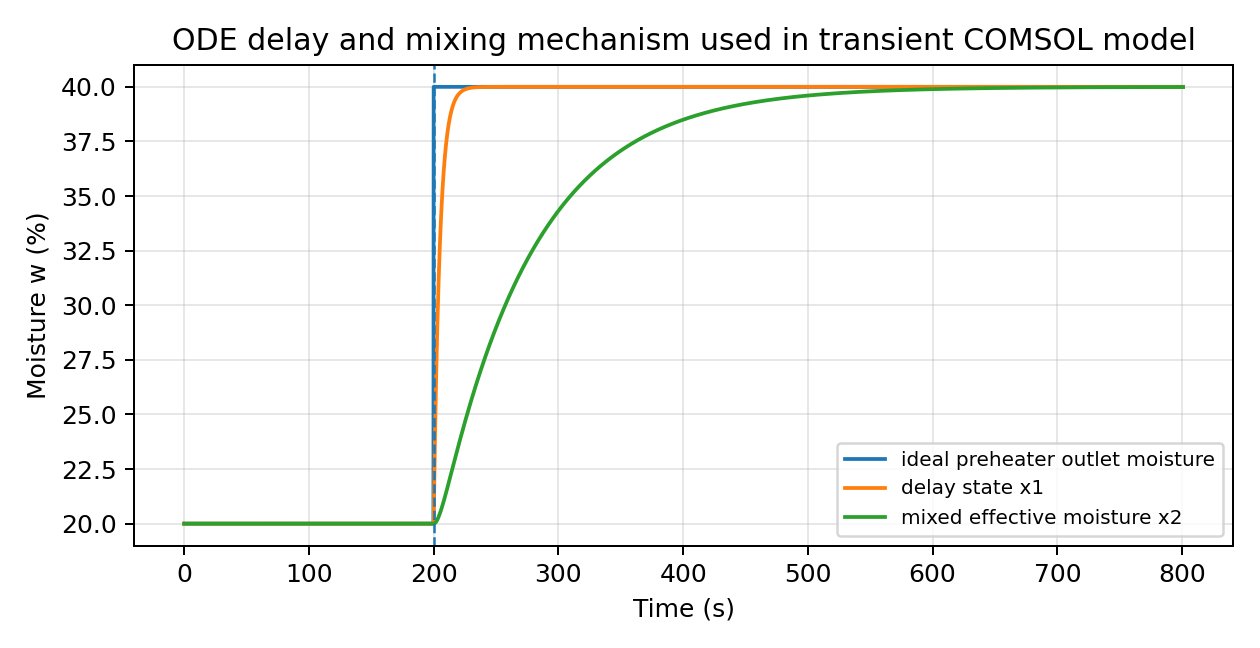
\includegraphics[width=0.86\textwidth]{transient_ode_moisture_response.png}
\caption{由 COMSOL 报告参数重构的含水率延迟与核心区混合响应}
\label{fig:ode-moisture-response}
\end{figure}

\begin{figure}[htbp]
\centering
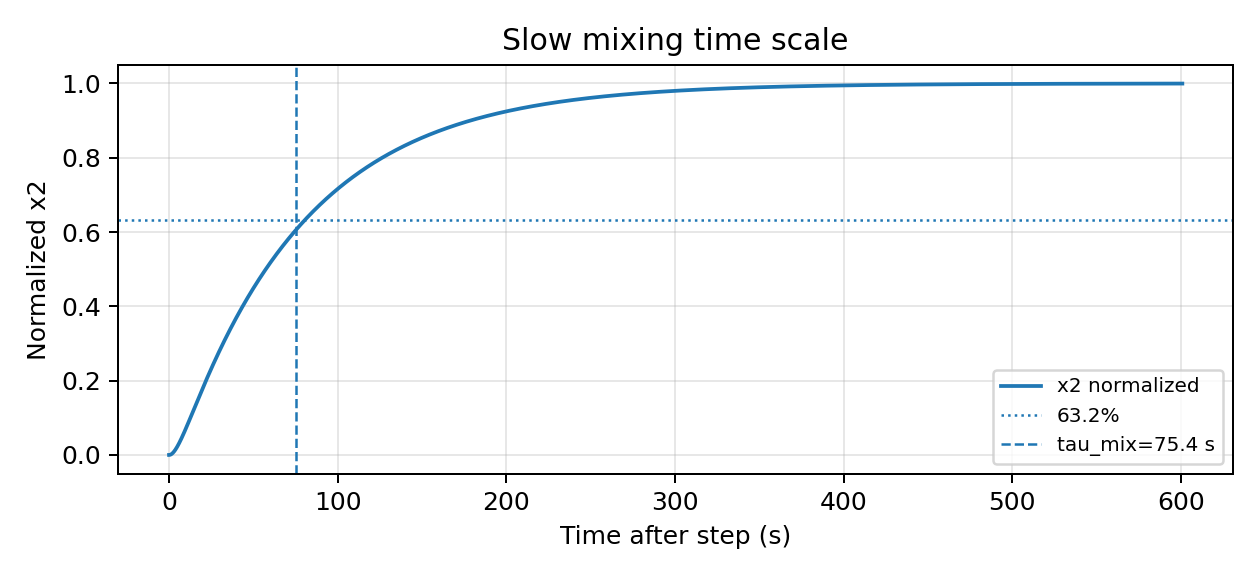
\includegraphics[width=0.82\textwidth]{transient_mixing_time_constant.png}
\caption{核心区混合环节的归一化响应与 \(\tau_{mix}=75.412\,\mathrm{s}\) 时间尺度}
\label{fig:mixing-time-constant}
\end{figure}

这一结果直接支持控制器中的“慢动态”设定：焚烧炉不会只对当前一拍入口含水率做出瞬时反应，而是对核心区内有效平均含水率做出反应。控制器预测器中应保留一个慢状态，用来描述进料库存和燃烧区混合造成的记忆效应。若后续将 COMSOL 结果拟合为低阶传递函数，\(\tau_{mix}\) 应作为慢时间常数的第一候选值；\(\tau_{trans}=5\,\mathrm{s}\) 则可作为进入炉膛前的短延迟或快惯性。


\section{热容效应验证}

热容效应材料采用了更完整的湍流与非等温流动设置，图 \ref{fig:heatcap-field-montage} 展示了温度、速度、压力、壁分辨率和耦合场结果。该实验证明了，在当前 100--600 s 的控制时间尺度上，炉体及固体热容影响几乎可以忽略不计。

\begin{figure}[htbp]
\centering
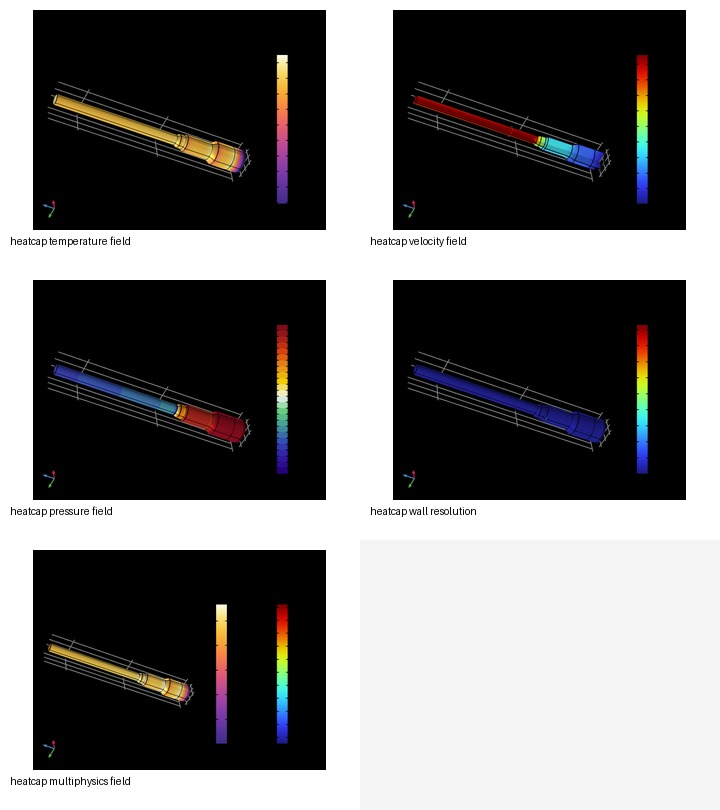
\includegraphics[width=0.92\textwidth]{heatcap_field_montage.jpg}
\caption{热容效应材料中的温度、速度、压力、壁分辨率和耦合场结果}
\label{fig:heatcap-field-montage}
\end{figure}

从报告导出的可比较体平均温度序列看，热容效应检查曲线与参考响应在导出精度下重合；按导出表格计算，两条可比较曲线的最大绝对差为 \(0.0^\circ\mathrm{C}\)。该结果说明，在当前模型设置和控制时间尺度下，显著影响焚烧炉动态的主要环节仍是入口含水率扰动的到达过程与燃烧区有效库存混合，而不是炉体热容单独引入的额外慢惯性。

\begin{figure}[htbp]
\centering
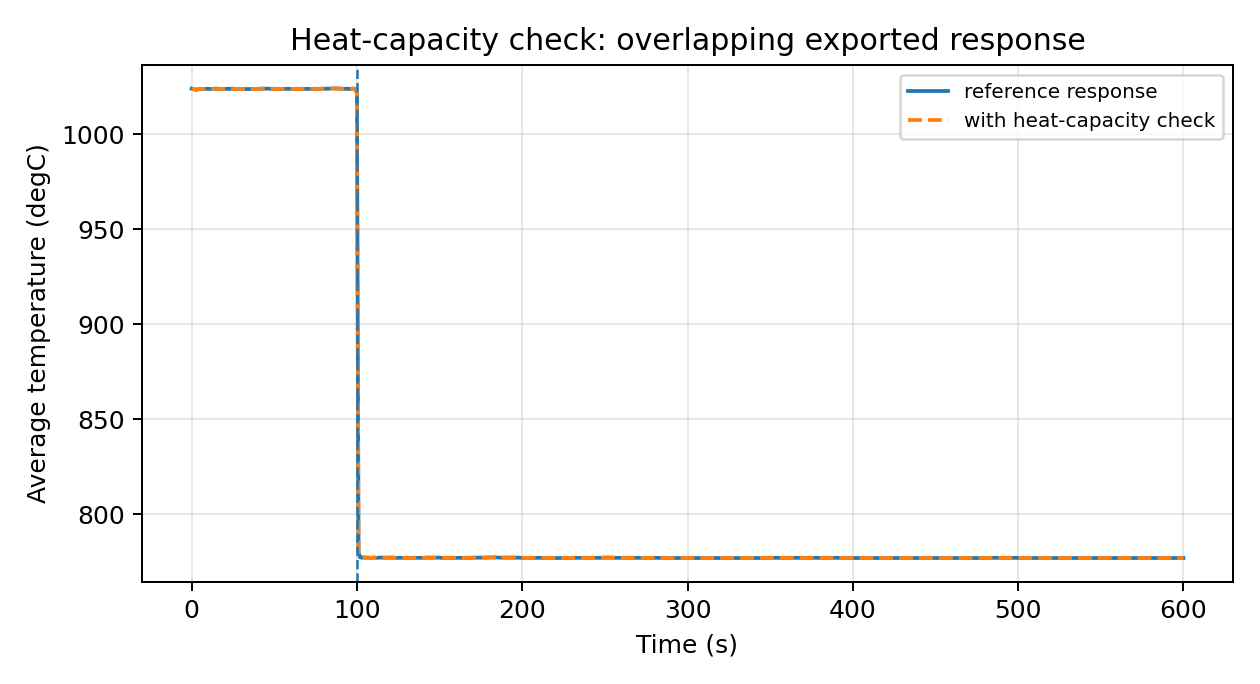
\includegraphics[width=0.86\textwidth]{heatcap_overlay.png}
\caption{热容效应检查中导出的可比较体平均温度响应曲线}
\label{fig:heatcap-overlay}
\end{figure}

\begin{figure}[htbp]
\centering
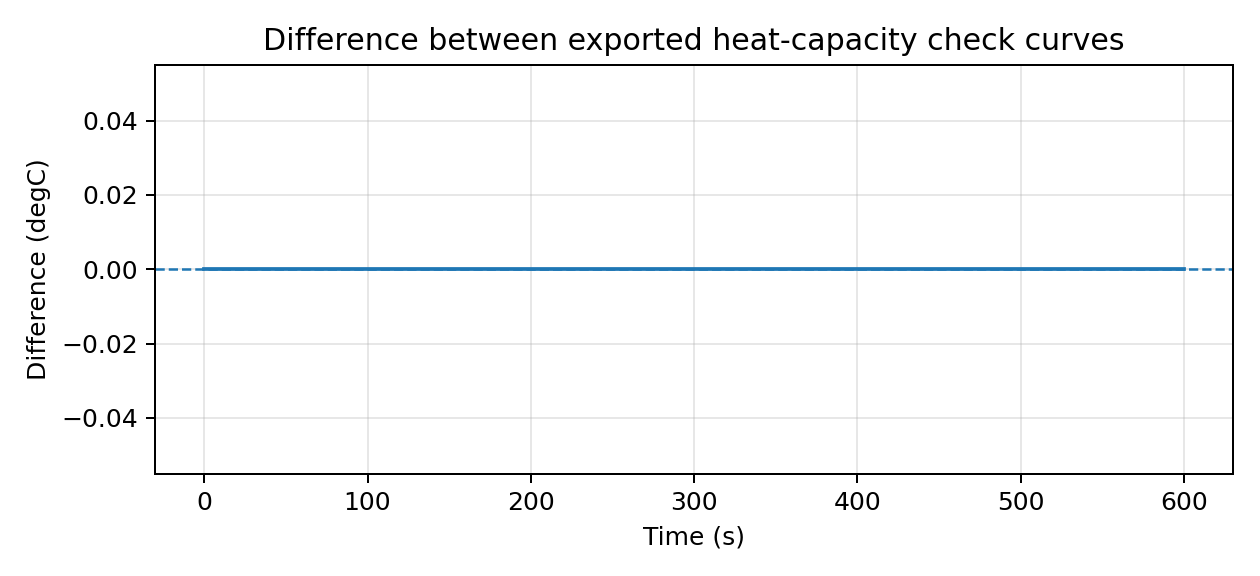
\includegraphics[width=0.82\textwidth]{heatcap_difference.png}
\caption{热容效应检查曲线与参考响应的差值}
\label{fig:heatcap-difference}
\end{figure}

该结论对控制器建模非常重要：如果炉体热容在该时间尺度上不构成主导动态，则不必在第一版 NMPC 预测器中引入高阶炉墙蓄热状态。更稳妥的做法是将热容效应作为安全裕度或二阶修正项处理，优先保证进料含水率、干基负荷、核心区混合和静态代理面的准确性。若后续扩展到更长时间尺度，例如连续运行数小时、启停炉或炉墙温度逐步漂移，则需要重新评估热容状态是否应进入控制器状态向量。

\section{结论与代码接入}

综合两份瞬态材料，可以给出以下建模结论。第一，静态代理模型仍是焚烧炉绝对稳态输出的标定来源；第二，瞬态材料证明入口含水率扰动应经过 \(\tau_{trans}=5\,\mathrm{s}\) 的短延迟和 \(\tau_{mix}=75.412\,\mathrm{s}\) 的核心区混合后再作用于等效体热源；第三，热容效应在当前控制时间尺度下不是主导动态，不宜为了它牺牲控制器模型的可辨识性和可解释性。

\begin{table}[htbp]
\centering\small
\begin{tabularx}{\textwidth}{p{35mm}p{38mm}X}
\toprule
模型项 & 建议取值/处理 & 说明 \\
\midrule
含水率输入 & \(w_{out}=w_0+\Delta w\,\mathrm{step}(t)\) & 用于激发焚烧炉热源变化，可替换为预热炉出口预测含水率。 \\
运输延迟/快惯性 & \(\tau_{trans}=5\,\mathrm{s}\) & 对应 \(w_{out}\rightarrow x_1\) 的快速环节。 \\
核心区混合慢惯性 & \(\tau_{mix}=75.412\,\mathrm{s}\) & 对应 \(x_1\rightarrow x_2\) 的有效库存混合，是当前最重要的慢动态来源。 \\
体热源输入 & \(Q=\dot m LHV(x_2)/V_{core}\) & 热源计算应使用 \(x_2\)，不直接使用理想阶跃 \(w_{out}\)。 \\
热容效应 & 第一版作为二阶修正或安全裕度处理 & 当前时间尺度下未形成新的主导动态；长时间运行工况另行验证。 \\
\bottomrule
\end{tabularx}
\caption{焚烧炉瞬态模型进入控制器的建议参数}
\end{table}

代码实现上，\pathcode{FurnaceDynConfig} 中：\(\tau_f\) 与进料到达延迟相关，慢时间常数与 \(M_{mix}/\dot m\) 相关。若后续重构 \pathcode{plant/python_model/furnace.py}，更推荐显式维护 \(x_1\) 和 \(x_2\) 两个状态，然后把 \(x_2\) 传入静态代理模型。

\manualdivider


\chapter{预热炉静态仿真与温度稳定性验证}

预热炉静态仿真的作用，是验证预热炉在给定烟气入口温度、入口速度和几何结构下能否形成稳定、连续且可用于控制器接口投影的温度场。与焚烧炉静态代理不同，本章关注预热炉本体结构、烟气侧湍流换热、多孔垃圾域传热以及外壁散热边界是否能够在稳态求解中闭合。当前 COMSOL 报告名称为“预热炉-稳态-多孔介质传热，湍流”，模型采用 SI 单位制，物理场包括多孔介质传热、湍流 SST 以及非等温流动耦合。

\notebox{注意}{目前的实验结果中可以获得给出几何、材料、边界条件、网格、稳态求解流程和结果场图，可以证明结构在给定工况下能够形成稳定的三维温度分布。但目前项目暂时未推进到完成出口截面平均温度、热平衡误差和壁面最高温度等派生值的建模与分析，也暂未完成将 COMSOL 预热炉模型作为独立后端接入控制器进行闭环验证的工作。}

\section{模型结构与基本工况}

预热炉计算域采用 3D 圆筒结构。炉体轴向长度为 \(L_g=3.2\ \mathrm{m}\)，炉体半径为 \(r_1=0.6\ \mathrm{m}\)，外壁半径为 \(r_3=0.7\ \mathrm{m}\)。六根导烟管围绕轴心均匀布置，导烟管半径为 \(r_2=0.084\ \mathrm{m}\)，管心位于半径 \(R_p=0.34\ \mathrm{m}\) 的圆周上。各导烟管中心位置由
\[
  y_i=R_p\sin\theta_i,\qquad z_i=R_p\cos\theta_i,\qquad
  \theta_i=0,\frac{\pi}{3},\frac{2\pi}{3},\pi,\frac{4\pi}{3},\frac{5\pi}{3}
\]
给出。几何联合体最终包含 16 个域、96 个边界、192 条边和 128 个顶点。该结构与《预热炉设计手册》中“多导烟管环绕垃圾通道进行间接换热”的工程思路一致。

\begin{table}[htbp]
\centering\small
\begin{tabularx}{\textwidth}{p{34mm}p{34mm}X}
\toprule
类别 & COMSOL 设置 & 手册解释 \\
\midrule
几何尺度 & \(L_g=3.2\ \mathrm{m}\), \(r_1=0.6\ \mathrm{m}\), \(r_3=0.7\ \mathrm{m}\) & 对应预热炉轴向长度、炉体半径和外壁半径。 \\
导烟管布置 & \(R_p=0.34\ \mathrm{m}\), \(r_2=0.084\ \mathrm{m}\) & 六根导烟管沿圆周均布，用于提高垃圾域周向受热均匀性。 \\
烟气入口 & \(T_{in}=673.15\ \mathrm{K}\), \(u_{in}=3\ \mathrm{m/s}\) & 约为 \(400^\circ\mathrm{C}\) 的热烟气，以法向速度进入导烟管入口。 \\
烟气出口 & \(p=0\ \mathrm{Pa}\)，抑制回流开启 & 出口采用相对压力边界，保证稳态流动方向稳定。 \\
外壁散热 & \(h=10\ \mathrm{W/(m^2\cdot K)}\), \(T_{ext}=293.15\ \mathrm{K}\) & 外壁通过对流热通量与环境换热，用于评价热损失和外壁温度分布。 \\
\bottomrule
\end{tabularx}
\caption{预热炉稳态 COMSOL 模型的主要参数与边界条件}
\end{table}

\begin{figure}[htbp]
\centering
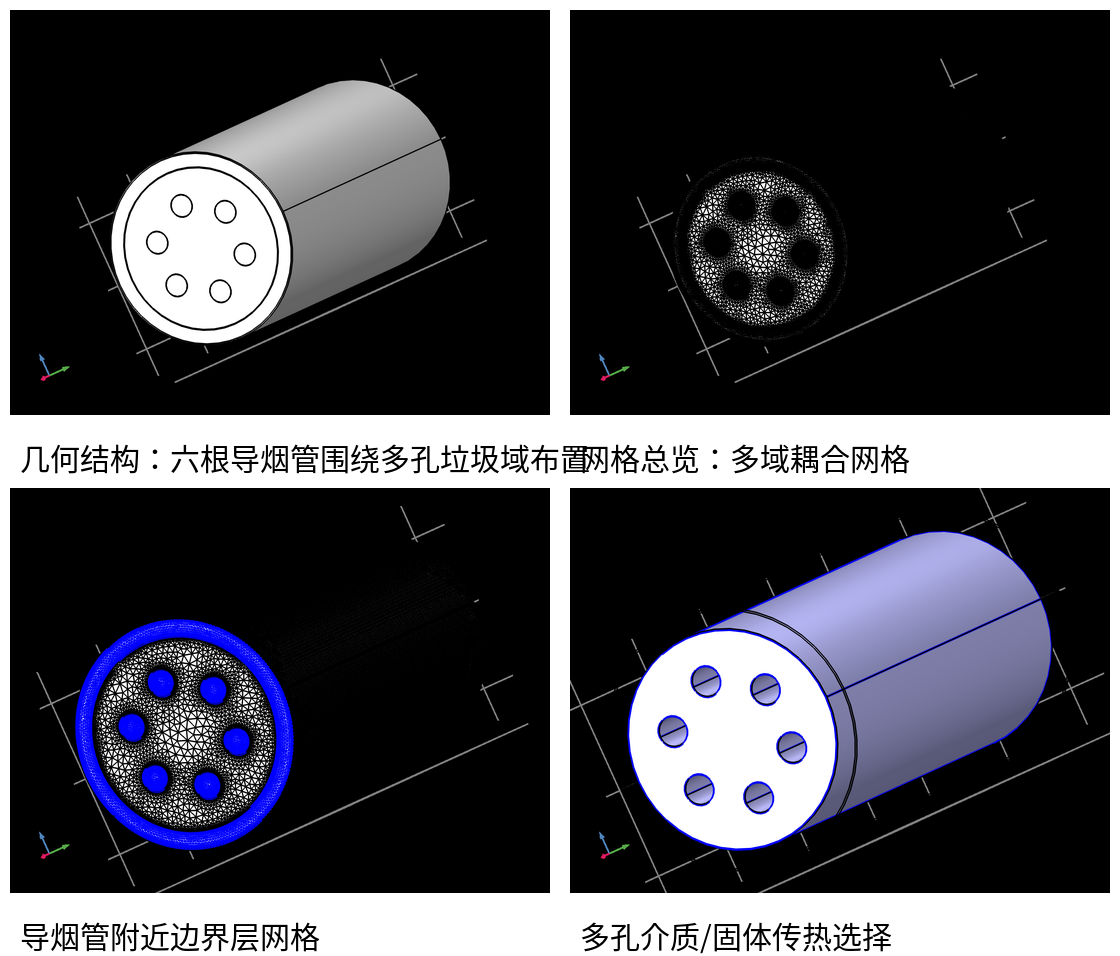
\includegraphics[width=0.94\textwidth]{preheater_geometry_mesh_montage.png}
\caption{预热炉稳态模型的几何、网格与多孔域设置}
\label{fig:preheater-geom-mesh}
\end{figure}

图 \ref{fig:preheater-geom-mesh} 中可以看出，几何模型已经区分了外壳、导烟管、管壁和中心多孔垃圾域。网格在导烟管和环形壁面附近进行了局部加密，并设置了边界层网格，这对于 SST 湍流模型和壁面换热计算是必要的。换言之，该模型不是简单的均匀热源模型，而是显式描述了烟气侧流动路径和壁面换热路径。

\section{材料与多物理场设置}

材料设置分为三类：烟气侧使用 Air，金属结构使用 304 不锈钢，多孔垃圾域使用“多相材料/多孔介质”表达。多孔基体采用局部热平衡假设，孔隙率为 0.6，干本体导热系数为 \(0.3\ \mathrm{W/(m\cdot K)}\)，干本体密度为 \(450\ \mathrm{kg/m^3}\)，干本体恒压热容为 \(3315\ \mathrm{J/(kg\cdot K)}\)。多孔域内流体按理想气体处理，导热系数为 \(0.036\ \mathrm{W/(m\cdot K)}\)，气体常数为 \(287\ \mathrm{J/(kg\cdot K)}\)，恒压热容为 \(1050\ \mathrm{J/(kg\cdot K)}\)。

\begin{table}[htbp]
\centering\small
\begin{tabularx}{\textwidth}{p{31mm}p{46mm}X}
\toprule
物理模块 & 主要设置 & 作用 \\
\midrule
多孔介质传热 & 局部热平衡；所有域参与传热计算 & 统一求解烟气、金属壁和多孔垃圾域的温度场。 \\
多孔基体 & \(\varepsilon=0.6\), \(k_s=0.3\), \(\rho_s=450\), \(C_{p,s}=3315\) & 将垃圾堆积层等效为多孔介质，表达其蓄热和导热能力。 \\
流体传热 & \(k_g=0.036\), \(R=287\), \(C_{p,g}=1050\) & 描述孔隙气体或烟气侧的热物性。 \\
湍流 SST & RANS-EVM，弱可压缩流动，自动壁处理 & 求解导烟管与环形通道中的高温烟气流动。 \\
非等温流动 & 湍流普朗特数模型 Kays--Crawford，标准热壁函数，黏性耗散开启 & 将速度场、压力场和温度场耦合，避免只做纯导热近似。 \\
\bottomrule
\end{tabularx}
\caption{预热炉稳态仿真的材料与多物理场设置}
\end{table}

注意，本实验目前采取的 COMSOL 模型中烟气入口温度为 \(673.15\ \mathrm{K}\)，即约 \(400^\circ\mathrm{C}\)，入口速度为 \(3\ \mathrm{m/s}\)。这不是控制器未来可选工况的全部边界，而是一个用于验证结构稳态传热与流动收敛性的基准工况。

\section{网格与稳态求解}

网格采用物理场控制网格，单元大小为常规。完整网格共包含 3,377,086 个单元，其中四面体单元 2,480,398 个、棱柱单元 896,688 个。最小单元质量为 0.06557，平均单元质量为 0.6765。导烟管和壁面附近采用边界层网格，层数为 6，厚度调节因子为 2。由于本模型同时包含 SST 湍流、非等温流动和多孔介质传热，导烟管壁面、入口、出口和外壁散热区域的网格质量直接影响稳态收敛和壁面换热结果。

\begin{table}[htbp]
\centering\small
\begin{tabularx}{\textwidth}{p{35mm}p{34mm}X}
\toprule
网格/求解项目 & 报告值 & 说明 \\
\midrule
总单元数 & 3,377,086 & 用于支撑多域耦合和导烟管附近速度梯度。 \\
四面体/棱柱单元 & 2,480,398 / 896,688 & 棱柱单元主要用于边界层和壁面附近梯度解析。 \\
最小/平均单元质量 & 0.06557 / 0.6765 & 局部最小质量偏低但整体平均质量可接受，后续参数扫描可保留重点区域加密。 \\
边界层 & 6 层，厚度调节因子 2 & 支持 SST 自动壁处理与壁面换热计算。 \\
研究步骤 & 壁距离初始化 + 稳态 & 先初始化壁距离，再进行稳态多物理场求解。 \\
\bottomrule
\end{tabularx}
\caption{预热炉稳态模型的网格与求解摘要}
\end{table}

\section{稳态结果与温度稳定性判断}

COMSOL 报告输出了温度场、速度场、压力场、壁分辨率以及非等温流动综合结果。温度场显示，高温主要集中在导烟管入口、管壁及外环换热侧，中心多孔垃圾域的温度分布呈连续梯度，没有出现孤立的高温斑点或明显数值振荡。速度场显示，烟气沿六根导烟管和环形通道形成稳定流动路径；压力场沿轴向呈连续变化；壁分辨率图用于检查 SST 自动壁处理是否有足够的网格支撑。

\begin{figure}[htbp]
\centering
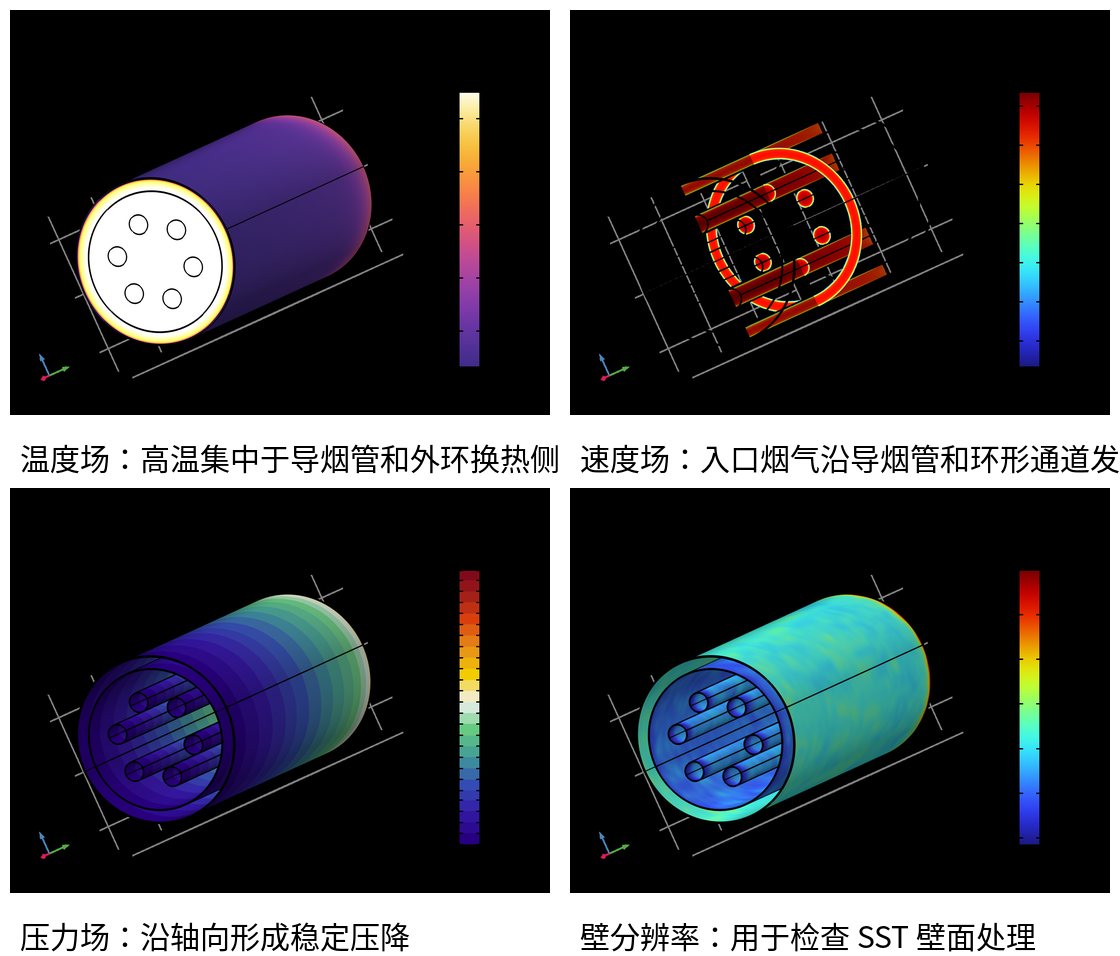
\includegraphics[width=0.94\textwidth]{preheater_result_fields_montage.png}
\caption{预热炉稳态仿真的温度、速度、压力与壁分辨率结果}
\label{fig:preheater-result-fields}
\end{figure}

从图 \ref{fig:preheater-result-fields} 可以得到三点结论。第一，烟气侧热量没有只停留在入口截面，而是沿轴向和周向传递，说明多导烟管布置能够形成有效换热路径。第二，中心垃圾域温度变化相对平滑，说明在当前入口温度和速度下，结构没有表现出强烈局部过热或温度场不连续问题。第三，速度和压力结果与入口速度、出口压力边界的设定相一致，未显示明显的大范围回流特征，因此可作为稳态预热温度稳定性的初步验证。

\begin{figure}[htbp]
\centering
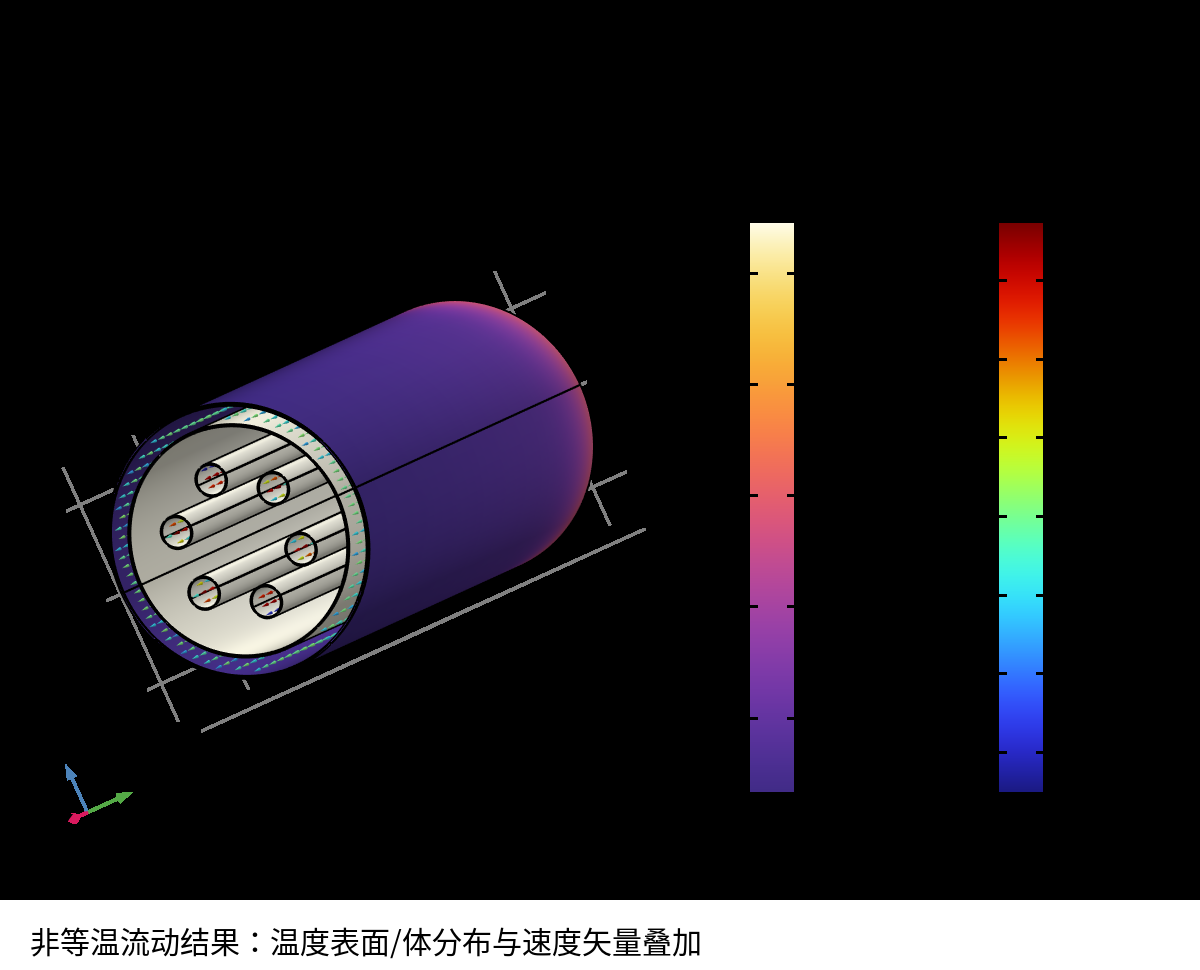
\includegraphics[width=0.88\textwidth]{preheater_temp_flow_labeled.png}
\caption{非等温流动耦合结果：温度分布与速度矢量叠加}
\label{fig:preheater-nitf}
\end{figure}

图 \ref{fig:preheater-nitf} 进一步说明，温度场和速度场在同一几何结构内是耦合求解的，而不是将烟气换热简化为固定壁温。因此，该结果可以支持“预热炉结构能够在稳态下形成稳定换热场”的判断。不过，由于当前报告没有导出出口截面平均温度、垃圾域体平均温度和热平衡误差，本章不能直接写成“出口预热温度已经达到某一具体数值”。更稳妥的表述是：当前 COMSOL 稳态报告已经证明该几何和物理场组合可以得到收敛且连续的稳态温度场，满足作为预热炉温度稳定性验证模型的基础要求。

\section{与低阶预热炉模型和控制接口的衔接}

在代码中，控制器并不直接使用完整三维温度场，而是使用 \pathcode{PreheaterOutput} 和 \pathcode{PreheaterState}。因此，预热炉 COMSOL 稳态结果需要投影为出口量和沿程量。最低要求是对出口截面和垃圾多孔域进行平均，得到：
\[
  T_{solid,out},\quad \omega_{out},\quad \dot m_{wet,out},\quad
  \dot m_{dry,out},\quad \dot m_{water,out},\quad T_{g,out}.
\]

综上，本次预热炉稳态 COMSOL 材料可以支撑手册中的以下结论：预热炉 3D 结构、多孔垃圾域、导烟管烟气流动和外壁散热边界能够在稳态多物理场中形成可收敛、连续且具有明确换热路径的温度场；该模型可作为后续预热炉参数扫描、出口温度验收和低阶模型校核的高保真基础。
\manualdivider

\end{document}
